\documentclass[12pt,a4paper,parskip]{scrreprt}
%parskip sorgt dafür, dass neue Absätze nicht automatisch eingerückt werden
\usepackage[utf8]{inputenc}
\usepackage[german]{babel}
\usepackage[T1]{fontenc}
\usepackage{amsmath}
\usepackage{amsfonts}
\usepackage{amssymb}
\usepackage{makeidx}
\usepackage{graphicx}
\usepackage{url}
\author{Markus Österle \\ Maximilian Schreiber \\ Tobias Schmidbauer \\ Stefan Memmel \\ Christoph Kammerer}
\title{Studienarbeit im Fach \\ \glqq Software Engineering 2\grqq}
\subtitle{Thema: Notenrechner}
%leeres Datum
\date{}
\makeindex
\setcounter{secnumdepth}{4}
\begin{document}
\maketitle
\tableofcontents
\chapter{Einleitung \& Motivation}
Die folgende Gruppenarbeit aus dem Fach \glqq Software Engineering 2\grqq\ beschäftigt sich mit einem für den Studiengang \glqq Verwaltungsinformatik\grqq\ tatsächlich relevanten Problem, durch die Aufteilung unseres Studiengangs auf zwei Hochschulen (FHVR AIV \& Hochschule Hof) und der damit verbundenen Aufteilung der Prüfungsleistungen, ergibt sich die Notwendigkeit einer zentralen Plattform, in die zum einen Noten eingetragen werden können (z.B. durch die Verwaltung oder auch berechtigte Dozenten) und zum anderen auch eingetragene Noten durch die Studierenden abgerufen werden können. Idealerweise soll bei dieser Gelegenheit auch eine Berechnung der Zwischen- und Endnoten erfolgen, um die im Studiengang kursierenden Exceltabellen durch eine rechtssichere und in jedem Fall richtig rechnende Plattform abzulösen.

Zur Realisierung einer solchen Plattform werden im folgenden Technologien eingesetzt, die im Rahmen der Lehrveranstaltungen 
\begin{itemize}
\item Objektorientiertes Programmieren 1 \& 2
\item Algorithmen und Datenstrukturen
\item Serverseitiges Programmieren mit Java
\item Software Engineering 1 \& 2
\end{itemize}
erlernt wurden. 

Details zu den eingesetzten Techniken finden sich in den folgenden Kapiteln.
\chapter{Lasten- und Pflichtenheft}
\section{Anforderungsliste}
In der ersten Sitzung unserer Projektgruppe wurde eine Anforderungsliste an das Projekt \glqq Notenrechner\grqq\ ausgearbeitet. Diese behandelt zu allererst Anforderungen aus zwei Sichten, auf der einen Seite Anforderungen, die die Verwaltung haben könnte und auf der anderen Seite Anforderungen der Studierenden. Diese Anforderungen wurde im Projektverlauf, wie in der Vorlesung gelernt, in ein Lasten- und Pflichtenheft umgearbeitet:
\subsection{Hochschule}
\begin{itemize}
\item Ortsunabhängiger Aufruf
\item Dozenten sollen von jedem Ort der Erde Noten einpflegen können
\item Dozenten können ihre Prüfungen aufrufen und auswerten
\item Ein Admin (Studiengangsleiter) soll die Gewichting der Noten ändern können
\item Admin soll Studiengänge modifizieren (wie z.B. Fächer zwischen den Semestern verschieben) und komplett neu anlegen können
\item Admin soll die Fähigkeit besitzen, neue Studenten anzulegen bzw. bestehende Studenten zu modifizieren (z.B. Namen ändern)
\item Statistik mit grafischer Aufarbeitung
\begin{itemize}
\item Aufruf von jedem, persönliche Einzelnoten können nur vom jeweiligen (angemeldeten) Studenten gesehen werden
\item Nachprüfungen werden wie Erstversuch behandelt
\item Möglichkeit Leistungsnachweise in die Prüfungsnote einrechnen oder nicht
\end{itemize}
\item Reminder (E-Mail Benachrichtigung) für Dozenten zur Eingabe der Prüfungsnoten (Mail 4 Wochen nach Prüfungsende)
\item Reminder für Studenten wenn neue Noten vorliegen (E-Mail)
\item Studiengang kann per Drag\&Drop zusammengestellt werden (durch den Studiengangsleiter)
\item Studiengang kann dupliziert und bearbeitet werden
\item Authentifizierung: Über vorhandene User (JAAS mit LDAP)
\begin{itemize}
\item benötigte Rollen:
\begin{itemize}
\item Dozent/Prüfungsamt
\begin{itemize}
\item kann nur Noten eintragen
\item seine Prüfungen einsehen
\end{itemize}
\item Studiengangsleiter (Admin)
\begin{itemize}
\item kann Gewichtung ändern
\item kann Personen hinzufügen/ändern
\item kann Studiengänge hinzufügen/ändern
\item kann Noten ändern (z.B. bei Fehlern)
\end{itemize}
\item Student
\begin{itemize}
\item Einsicht Wunsch-/Traumnoten
\end{itemize}		
\end{itemize}
\end{itemize}
\end{itemize}
\subsection{Student}
\begin{itemize}
\item Reminder, wenn neue Noten eingetragen wurden
\item Wunschnoten können eingetragen werden und werden überschrieben, wenn \glqq echte\grqq\ Noten vorhanden sind ODER \glqq echte\grqq\ Noten stehen neben den Traumnoten
\item Statistik (farblich aufbereitet in der Notenübersicht, z.B. grün = über dem Durchschnitt \& bestanden, rot = durchgefallen, gelb = bestanden, aber unter dem Durchschnitt)
\item Ortsunabhängiger Abruf
\item Übersicht über nicht bestandene Klausuren bzw. unterpunktete Leistungsnachweise
\item Zwischennoten (welche Noten hatte ich in der Zwischenprüfung?), Anzeige welche Noten noch notwendig sind um zu bestehen (Leistungsnachweise)
\end{itemize}
\subsection{Zusammenfassung Anforderungen}
Noch notwendig????
\begin{itemize}
\item 2 Frontends (Verwaltung \& Studierende)
\item individualisierbare Notenliste/-berechnung pro Jahrgang
\item Studiengangspezifisch, d.h. Programm nur für Vinf oder allgemeingültig?
\item Wenn allgemeingültig müsste der Administrator in der Lage sein Studiengänge mit Spezifikation zu erstellen - kann schwierig werden

\item Ablage der Noten in einer Datenbank -> Diskussionsbedarf, SQL oder NoSQL
\item Generierung von Testdaten (Mock data) für die Datenbank
\begin{itemize}
	\item Ist möglich durch CSV Dateien der ersten Semester
\end{itemize}
\item Ablage der Noten kann nur durch den Administrator/Dozenten erfolgen
\item graphische Aufbereitung der Noten in Diagrammen
\item statistische Kennzahlen berechen (Standartabweichung, Durchschnittsnote,...)
\item Statistikfunktionen für den Jahrgang
\item Farbliche Abhebung der Noten, ob durchgefallen (rot), über- (grün)/unterdurchschnittlich (gelb) usw...
\item Durchschnittsnote für alle sichtbar (kann bedenklich sein wenn nur zwei Studenten das Fach geschrieben haben)
\item Authentifizierung notwendig über JAAS
\item Desktop Client mit JavaFX (optional?)
\item Umsetzung in \glqq gesprochene Noten\grqq\ (sehr gut, gut, usw...)
\item Eintragung von \glqq Traumnoten\grqq\ der Studenten und anschließende Berechnung der \glqq resultierenden/prognostizierenden\grqq\ Endnote, die überschrieben werden durch Eintragung der echten Note durch den Dozenten
\item Technologie fuer die Abhängigkeitsverwaltung?
\begin{itemize}
\item Ant
\item Maven
\item Gradle
\end{itemize}
\item Mobile Devices über App oder AngularJS? Wenn App, welche Plattformen?
\end{itemize}
\section{Lastenheft}
\subsection{Zielbestimmung}
Es soll eine Software entwickelt werden, die eine einfache Eingabe und Berechnung von Noten gemäß der gesetzlichen Bestimmungen erlaubt. Die Software soll sowohl von der Verwaltung intern, als auch von den Studierenden benutzt werden. Ein geeignetes Berechtigungsmodell muss implemetiert werden. Die Software soll von überall abrufbar sein, maximal portierbar sein und somit auf möglichst vielen Plattformen abgerufen werden können.
\subsection{Produkteinsatz}
Der Einsatz des Produktes ist auf einem zentralen Server der FHVR vorgesehen. Dieser Server soll nur über das \glqq FHVR Intranet\grqq\ erreichbar sein. Die Authentifizierung soll im Endausbau über bereits vorhandene AD (Active Directory) Konten realisiert werden.
\subsection{Produktübersicht}
Es soll ein Webservice mit mindestens zwei voneinander getrennten Oberflächen geschaffen werden. Der Zugang zu den Oberflächen soll sich nach den Benutzern zugeordneten Rollen richten. Es sind mindestens drei Rollen vorzusehen:
\begin{itemize}
\item Studierende
\item Dozenten
\item Administrator
\end{itemize}
Für die Speicherung der Noten ist eine geeignete performante Speichermethode vorzusehen (bspw. SQL oder NoSQL).
Nach Möglichkeit soll für die Realisierung Software eingesetzt werden, für die keine Lizensierungskosten anfallen und deren Wartbarkeit und Sicherheit trotzdem auf absehbare Zeit gesichert ist.
\subsection{Produktfunktionen}
Es sind folgende Funktionen vorzusehen:
\begin{itemize}
\item Persistente Speicherung der Daten mithilfe einer geeigneten Technologie
\item Eingabe von Prüfungsleistungen
\item Für Studierende ist die Möglichkeit der Eingabe von \glqq Wunschnoten\grqq\ vorzusehen, diese sollen genau wie die \glqq echten\grqq\ Noten behandelt werden, d.h. gespeichert werden und es sollen aus diesen Werten die Zwischen- und Endnoten berechnet werden.
\item Farbliche Markierung für Notenwerte, die im Grenzbereich und unterhalb der Anforderungen liegen (niedrige Priorität), sodass für die Studierenden auf einen Blick zu erfassen ist, wie ihre Leistungen einzustufen sind
\item Berechnung muss entsprechend der gesetzlichen Vorgaben umgesetzt werden
\item Die Anwendung soll modular gehalten werden, d.h. es sollen komplett neue Studiengänge angelegt werden können
\item Benutzeroberfläche soll Plattformunabhängig sein, dies umfasst auch mobile Endgeräte. Die Oberfläche ist so auszulegen, dass sie auch auf mobilen Endgeräten bedient werden kann.
\item Authentifizierungstechnologie muss vorhandenes Active Directory (AD) unterstützen
\item Rollenbasiertes Zugriffsmodell, die Zuordnungen zu den Rollen sollen aus dem AD übernommen werden. 
Es sind 3 Rollen mit den folgenden Berechtigungen vorzusehen:
\begin{itemize}
\item Administrator
\begin{itemize}
\item Anlegen von neuen Studiengängen (inkl. Eingabe der abzulegenden Prüfungsleistungen und Notengewichtung)
\item Modifizieren von vorhandenen Studiengängen
\item Eintragung von Noten (ohne Beschränkungen auf bestimmte Fächer)
\item Anlegen von neuen Nutzern (sofern nicht automatisch realisiert)
\item Vergabe der Berechtigungen für Dozenten (Zuteilung der Fächer)
\end{itemize}
\item Dozenten
\begin{itemize}
\item Eintragen von abgelegten Prüfungsleistungen für zugewiesene Fächer
\item Abruf der aus den eingetragenen Prüfungsleistungen berechneten Statistiken
\end{itemize}
\item Studierende
\begin{itemize}
\item Eintragen von Wunschnoten, diese sind genauso zu behandeln wie eingetragene \glqq Echtnoten\grqq
\item Abrufen bereits abgelegter Prüfungsleistungen und (daraus) berechneter Zwischen- und Endnoten
\item Abruf statistischer Daten (Durchschnitt, Median, etc.) zu den eingepflegten Prüfungsleistungen
\end{itemize}
\end{itemize}
\end{itemize}
\subsection{Produktdaten}
\subsection{Produktleistungen}
Das Produkt stellt eine Plattform zur Verfügung, auf der aus eingegeben Prüfungsleistungen Statistiken abgeleitet werden, die eine geordnete und berechnete Ausgabe zur Verfügung stellt.
\subsection{Qualitätsanforderungen}
Es ist sicherzustellen, dass die angebotene Software die Noten entsprechend der gesetzlichen Vorgaben richtig berechnet. Der Datenschutz muss in jeder Betriebssituation gewahrt sein.
Es ist sicherzustellen, dass die benutzten Technologien und Programme in den nächsten Jahren noch Weiterentwicklung und Support bekommen.
\subsection{Ergänzungen}
\section{Pflichtenheft}
\subsection{Zielbestimmung}
\subsubsection{Musskriterien}
\begin{itemize}
\item Authentifizierung (vorerst noch nicht per LDAP)
\item Oberfläche für Studierende mit Abfrage der Noten und Möglichkeit zur Eingabe der Wunschnoten
\item Oberfläche für Dozenten mit der Möglichkeit Prüfungsleistungen einzugeben
\item Plattformunabhängigkeit
\end{itemize}
\subsubsection{Wunschkriterien}
\begin{itemize}
\item Farbliche Markierung der Prüfungsleistungen
\item Mobile Oberfläche
\item Eigene Anwendung zur Verwendung auf Desktop PCs (Desktop Client)
\item Anlegen von komplett neuen Studiengängen mit eigenen Fächern und Gewichtungen der Prüfungsleistungen durch den Administrator
\item Bereits geschriebene Note automatisiert als Wunschnote eintragen (Oberfläche für Studierende)
\end{itemize}
\subsubsection{Abgrenzungskriterien}
\subsection{Produkteinsatz}
\subsubsection{Anwendungsbereiche}
\subsubsection{Zielgruppen}
Zielgruppe der Anwendung sind im wesentlichen die Studierenden und die Dozenten der Hochschulen. Die Verwaltung der FHVR als Dienstherr der Verwaltungsinformatiker ist von eher untergeordneter Bedeutung für die Entwicklung, da diese einen zahlenmäßig sehr kleinen Teil der gesamten Nutzerschaft ausmacht.
\subsubsection{Betriebsbedingungen}
\subsection{Produktumgebung}
\subsubsection{Software}
Um die Kosten für Lizenzen und Support möglichst gering zu halten, wird der Einsatz von Linux als Serverbetriebssystem empfohlen, als Datenbank wird MySQL oder MariaDB empfohlen und als Applicationserver soll Wildfly in einer aktuellen Version zum Einsatz kommen.
\subsubsection{Hardware}
Das Produkt ist auf allen Plattformen lauffähig, die die benötigten Softwareprodukte unterstützen, neben x86\_64 also bspw. auch SPARC und ARMv6/v7/v8.
\subsubsection{Orgware}
TODO: Sicherheitsanforderungen, Benutzerhandbücher
\subsubsection{Produkt – Schnittstellen}
\begin{itemize}
\item LDAP als Schnittstelle zum vorhandenen Active Directory (AD)
\end{itemize}
\subsection{Produktfunktionen}
\subsubsection{Produktspezifisch}
\subsection{Produktdaten}
\subsubsection{Produktspezifisch}
\subsection{Produkt - Leistungen}
\subsection{Benutzungsoberfläche}
Als Benutzeroberfläche kommt im ersten Entwicklungsschritt die Web Technologie Java Server Faces (JSF) zum Einsatz. In weiteren Entwicklungsschritten ist angedacht eine (lokale) Java Application mit einer JavaFX Oberfläche zur Verfügung zu stellen.
\subsection{Qualitäts-Zielbestimmung}
\subsection{Globale Testszenarien/Testfälle}
\subsection{Entwicklungsumgebung}
Als Java (EE) - Entwicklungsumgebung kommt Netbeans in der Version 8.1 zum Einsatz.

Für die Entwicklung der Datenbankschemata und Skripte wird die MySQL Workbench in der Version 6.3 zum Einsatz kommen.

Als Testumgebung wird eine virtuelle Maschine auf Suse Linux Basis verwendet. 
\subsection{Ergänzungen}
\subsection{Glossar, Begriffslexikon}
\chapter{Verwendete Technologien}
Im ersten Meeting (Kick-Off meeting) des Teams wurden die zu verwendenden Softwareversionen festgelegt. Diese wurden im Verlaufe des Projekts nur noch aufgrund äußerer Begebenheiten (bekannte Fehler mit Fix in höherere Version, finale Version) angepasst. Die jeweils festgelegte Version und warum diese unter Umständen noch angepasst wurde, findet sich im jeweiligen Unterpunkt.
\section{Entwicklung}
\subsection{Java SDK}
Als Java Umgebung kam während der ganzen Projektdauer das Oracle Java SDK Version 8 Update 60 zum Einsatz.
\subsection{Entwicklungsumgebung - Netbeans}
festgelegte Version: \textbf{8.1RC2}\\
während des Projektverlaufs verändert? \textbf{ja}\\
Grund: \textbf{erscheinen der finalen Version} \\
geändert zu Version: \textbf{8.1 final}\\

\subsection{SQL Editor - MySQL Workbench}
\subsection{Versionsverwaltung - GIT}
Als Versionsverwaltung und zum Austausch des aktuellen Versionsstand des Projektes wurde während des gesamten Projektes Git eingesetzt. Das zentrale Repository liegt auf Github:
\url{https://github.com/themanwhosold/notenrechner}
\subsection{Bibliotheksverwaltung mit Maven}
%TODO Markus schreibt
Der Name \textit{Maven} kommt aus dem Jiddischen und bedeutet
\glqq Sammler des Wissens\grqq \footnote{\url{https://de.wikipedia.org/wiki/Apache_Maven}}.
\textit{Maven} ist eigentlich ein Build Management Tool und hat einen wesentlichen größeren Funktionsumfang als der der für das Projekt benutzt wurde.
\section{Test}
\subsection{Unit Tests mit JUnit}
Als Unit-Test Framework wurde JUnit eingesetzt und Testpackages für jede Klasse erzeugt. In diesen Testklassen wurden Testfälle definiert und bei jedem Build auf korrektheit überprüft. Hierdurch wurde sichergestellt, dass neu hinzugekommene Funktionalitäten nicht die Funktionsfähigkeit bereits vorhandener Komponenten verändert.
Weiterhin wurde für den Test der Java EE Webanwendung Mockito in Verbindung mit Arquillian eingesetzt, da zur Laufzeit die jeweilige Unit getestet werden muss. Hierdurch können die Schnittstellen der jeweiligen Objekte definiert und angesteuert werden.
\subsection{Continous Integration Tests mit Travis, Jenkins und Sonarqube}
%TODO Markus schreibt
Um einen möglichst fehlerfreien Master Zweig zu erhalten wurden Pull Requests nur nach fehlerfreiem Durchlauf der beiden CI Tools Travis \& Jenkins in den Master Zweig übernommen.

\subsubsection{Travis}
Travis\footnote{\path{https://travis-ci.org/}} wird von Github als Tool für CI angeboten, das macht die Integration in die Github Oberfläche sehr einfach, man muss sich nicht mit Hooks und Anmeldeinformationen rumschlagen und bei Bearbeitung eines Pull Requests ist auf einen Blick der Status des Travis Builds sichtbar.
\begin{figure}[!hbtp]%
\centering
\includegraphics[width=1\linewidth]{pics/screenTravis}
\caption[Travis]{Screenshot eines Travis Builds}
\label{fig:screenTravis}
\end{figure}
\subsubsection{Jenkins}
Jenkins wurde als zweites CI Tool eingesetzt
\begin{figure}[!hbtp]%
\centering
\includegraphics[width=1\linewidth]{pics/screenJenkins}
\caption[Jenkins]{Jenkins Screenshot}
\label{fig:screenJenkins}
\end{figure}
\subsubsection{Sonarqube}
Zur Analyse der Codequalität wurde Sonarqube\footnote{\path{http://www.sonarqube.org/}}\footnote{\path{https://de.wikipedia.org/wiki/SonarQube}} eingesetzt, die Analyse wurde von Jenkins bei jedem Build angesteuert. Sonarqube ist auf dem selben Server installiert wie Jenkins und liefert keinerlei Werte zurück an Git (anders als Jenkins selbst).
\begin{figure}[!hbtp]%
\centering
\includegraphics[width=1\linewidth]{pics/screenSonarqube}
\caption[Sonarqube]{Sonarqube Screenshot}
\label{fig:screenSonarqube}
\end{figure}
\section{Betrieb}
%TODO Markus schreibt
\subsection{Wildfly}
\subsection{MySQL}
\section{Übersicht über die final verwendeten Versionen}
\begin{center}
\begin{tabular}{|c|c|}
\hline
\rule[-1ex]{0pt}{2.5ex} Software & Version  \\ 
\hline 
\rule[-1ex]{0pt}{2.5ex} Oracle Java SDK & 8u60  \\ 
\hline 
\rule[-1ex]{0pt}{2.5ex} Java EE & 7 \\ 
\hline 
\rule[-1ex]{0pt}{2.5ex} Netbeans & 8.1 \\ 
\hline 
\rule[-1ex]{0pt}{2.5ex} MySQL &  \\ 
\hline 
\rule[-1ex]{0pt}{2.5ex} MySQL Workbench & 6.3 \\ 
\hline
\rule[-1ex]{0pt}{2.5ex} Wildfly Application Server & 9.0.1 \\ 
\hline 
\end{tabular}
\end{center}
\chapter{Teamstruktur und Arbeitsverteilung}
\section{Gemeinsame Codeentwicklung mit GIT}
Es wurde gegen ein gemeinsames Github-Repository entwickelt, von dem sich jeder im Team einen eigenen Fork erstellt hat. Entwickelter Code wurde per Pull Request an den Eigner des Hauptrepositories geschickt und von diesem nach erfolgreichen CI-Tests in den Hauptzweig gemerged. Diese Vorgehensweise hat sich nach einigen anfänglichen Schwierigkeiten als die sicherste herausgestellt, da Code, der zu Fehlern im Build-Prozess führt, vor dem Zusammenführen erkannt und nachgebessert werden kann und somit nicht der komplette Master-Branch unbrauchbar bzw. fehlerhaft wird.
\section{Arbeitsverteilung}
Es wurde angedacht das Projekt im Scrum Verfahren zu entwickeln. Jedoch wurde schnell klar, dass die Programmierfähigkeiten aller Teammitglieder und die Erfahrung mit Programmierobjekten nicht ausreichen um dies umzusetzen.
Die im Kickoff-Meeting festgelegten Anforderungen wurden in einem Lasten- und Pflichtenheft festgehalten und dienten als Grundlage der Entwicklungsarbeiten. In den wöchentlichen Meetings wurden von den Teammitgliedern Themen ausgewählt und soweit möglich bis zum nächsten Meeting realisiert. Die Ergebnisse wurden vorgestellt und sofern noch Ergänzungsbedarf oder Fragen bestanden ergänzt oder zusammen mit einem anderen Mitglied weiterentwickelt.

Zur Abstimmung des Codes wurde von jedem Teamangehörigen ein Repository auf Git verwaltet, nach erledigter Programmiertätigkeit wurde der geänderte Code per Pull Request in das Master Repository übertragen, wo es nach einem kurzen Review gemerged wurde.

Nachdem im Gesamtprojekt eine gewisse Codequalität erreicht wurde, wurde der Code von einem Teammitglied, das nicht an der Entwicklung der jeweiligen Passagen beteiligt war refactored und überarbeitet.
\subsection{Protokolle der wöchentlichen Meetings}
<<<<<<< HEAD
Wöchentliche \glqq Sprint\grqq\ Meetings auf denen die Fortschritte, aufgetretene Probleme und Lösungen besprochen werden und bei Bedarf neue Aufgaben verteilt werden. Leider ist die Protokollierung dieser Meetings nur sehr lückenhaft erfolgt. Die vorhandenen Protokolle finden sich aber in Folge.
=======
Wöchentliche \glqq Sprint\grqq\ Meetings auf denen die Fortschritte, aufgetretene Probleme und Lösungen besprochen werden und bei Bedarf neue Aufgaben verteilt werden.
>>>>>>> Sequenzdiagramme ergänzt
\subsubsection{Kickoff Meeting}
Protokoll siehe Punkt 2.1 Anforderungsliste
\subsubsection{2tes Meeting}
Beginn der Programmierarbeiten
Verfeinerung der Anforderungen an die Maske für den Administrator:
Maske für den Admin:
\begin{itemize}
	\item Neuen Studiengang anlegen
	\item Wieviele Semester hat Studium
	\item Welche Semester = Grundstudium, Ausschlußprinzip alle anderen gehören zum Hauptstudium
	\item Stellenwert des Grundstudiums in der Endnote, Ausschlußprinzip -> Hauptstudium
	\item Studienfächer zum Grundstudium hinzufuegen
	\item zu vergebende Noten \& Art der Noten festlegen
	\item Gewichtung festlegen (Noten untereinander \& Leistungsnachweise zu normalen Noten)
	\item Art der Noten (FHVR Klausur, FH Klausur, FH Leistungsnachweis, FHVR Leistungsnachweis) vs. jede Note einzeln eintragen
	-> Art der Noten (extra Tabelle), jeweils für Grund- und Hauptstudium
		\begin{itemize}
		\item FHVR Klausur
		\item FH Klausur
		\item FHVR Leistungsnachweis
		\item FH Leistungsnachweis
		\item FH Mündl. Prüfung
		\item FHVR Mündl. Prüfung
		\item FHVR Studienarbeit
		\item Praxisbeurteilung
		\end{itemize}
	\item Notentyp | Studienjahr | Gewichtung GS | Gewichtung HS
\end{itemize}
\subsection{weiteres Protokoll}
\underline{Bisheriger Arbeitsstand:}
\begin{itemize}
	\item es fehlen noch große Teile der Dokumentation
\item Stefan erstellt Diagramme (Stefan)
\item Lasten-/Pflichtenheft (Markus)
\item Voraussetzung/Installationsanleitung (Markus)
\item Ergänzung der Javadocs (Tobias)
\item Administratorseite:
\item Anlegen eines neuen Studenten in einem vorhandenen Studiengang (Max)
\item Notenberechnung:
\item Durchschnittsnoten der Leistungsnachweise sind nicht korrekt
\item Datenmodell müsste feingranularer werden (8 verschiedene Gewichtungen)			- mgl. Lösung zusätzliche Boolean Werte in der Notenliste
\item Enum für Umrechnung von Notenpunkten in gesprochene Noten (Christoph)
\end{itemize}
\chapter{(realisierte) Funktionalitäten}
Hier sollen die Ablaufdiagramme hin
Realisierung der Statistik-Funktionen:
Dazu wird eine zentrale Java Enterprise Bean genutzt. Die Session-Bean StatistikBean übernimmt die Analyse der empirischen Daten. Die Bean stellt alle gängigen statistischen Kennzahlen zu Verfügung.
Folgende statistische Maßzahlen werden berechnet:
- Median
- arithmetisches Mittel
- Beste und schlechteste Note
- Varianz
- Standartabweichung

Die in StatistikBean implementierte Methode getStatistik(int idStudienfach) benötigt als Übergabeparameter die Id des zu analysierenden Studienfaches. Daraufhin werden alle Noten des jeweiligen Studiengangs aus der MySql Datenbank abgefragt. Diese Liste von Noten werden im folgenden analysiert und die oben gennanten statistischen Kennzahlen berechnet. Die Methode liefert ein Objekt der Klasse Statistik zurück, die die Werte der Berechnungen enthält.


Realisierung der Berechnung der End- bzw. Zwischennoten:

Die Logik zur Berechnung der Noten stellt die Java Enterprise Bean BerechnungNoten bereit. Die Berechnung findet für jeden Studenten individuell auf Basis der in der Datenbank persitierten Daten statt. 
Dazu ist die Methode getEndnote(int matrikelNr) in der Bean implementiert. Diese erwartet als Übergabeparameter den Primärschlüssel matrikelNr, um die Noten des jeweiligen Studenten aus der Datenbank abzufragen. Daraufhin werden die Noten zusammengerechnet und die Zwischen- und Endnote zu ermitteln.
Zunächst wird eine Zwischennote (Note nach der Zwischenprüfung) berechnet. Daraufhin wird die Endnote ermittelt.

Die Methode getEndnote(int matrikelNr) liefert ein Objekt der Klasse Endnote zurück, die die Werte der Berechnungen enthält. Die Klasse Endnote enthält immer zwingend eine Zwischenprüfungsnote. Dadurch ist gewährleistet, dass auch die Zwischenprüfungsnote dem Studenten mitgeteilt werden kann.
\section{Oberfläche für Studierende}
\subsection{Funktionsumfang}
%TODO ausformulieren
\subsection{UML-Diagramm}
\section{Oberfläche für Dozenten}
\subsection{Funktionsumfang}
\section{Oberfläche für den Administrator}
\chapter{Einsatz der Software}
\section{Systemvoraussetzungen}
\section{Installation}
\chapter{Diagramme}
Auf den folgenden Seiten finden sich einige UML Diagramme, diese finden sich in Originalgröße auf der 
\section{UML Diagramme}
\begin{figure}[!hbtp]%
\centering
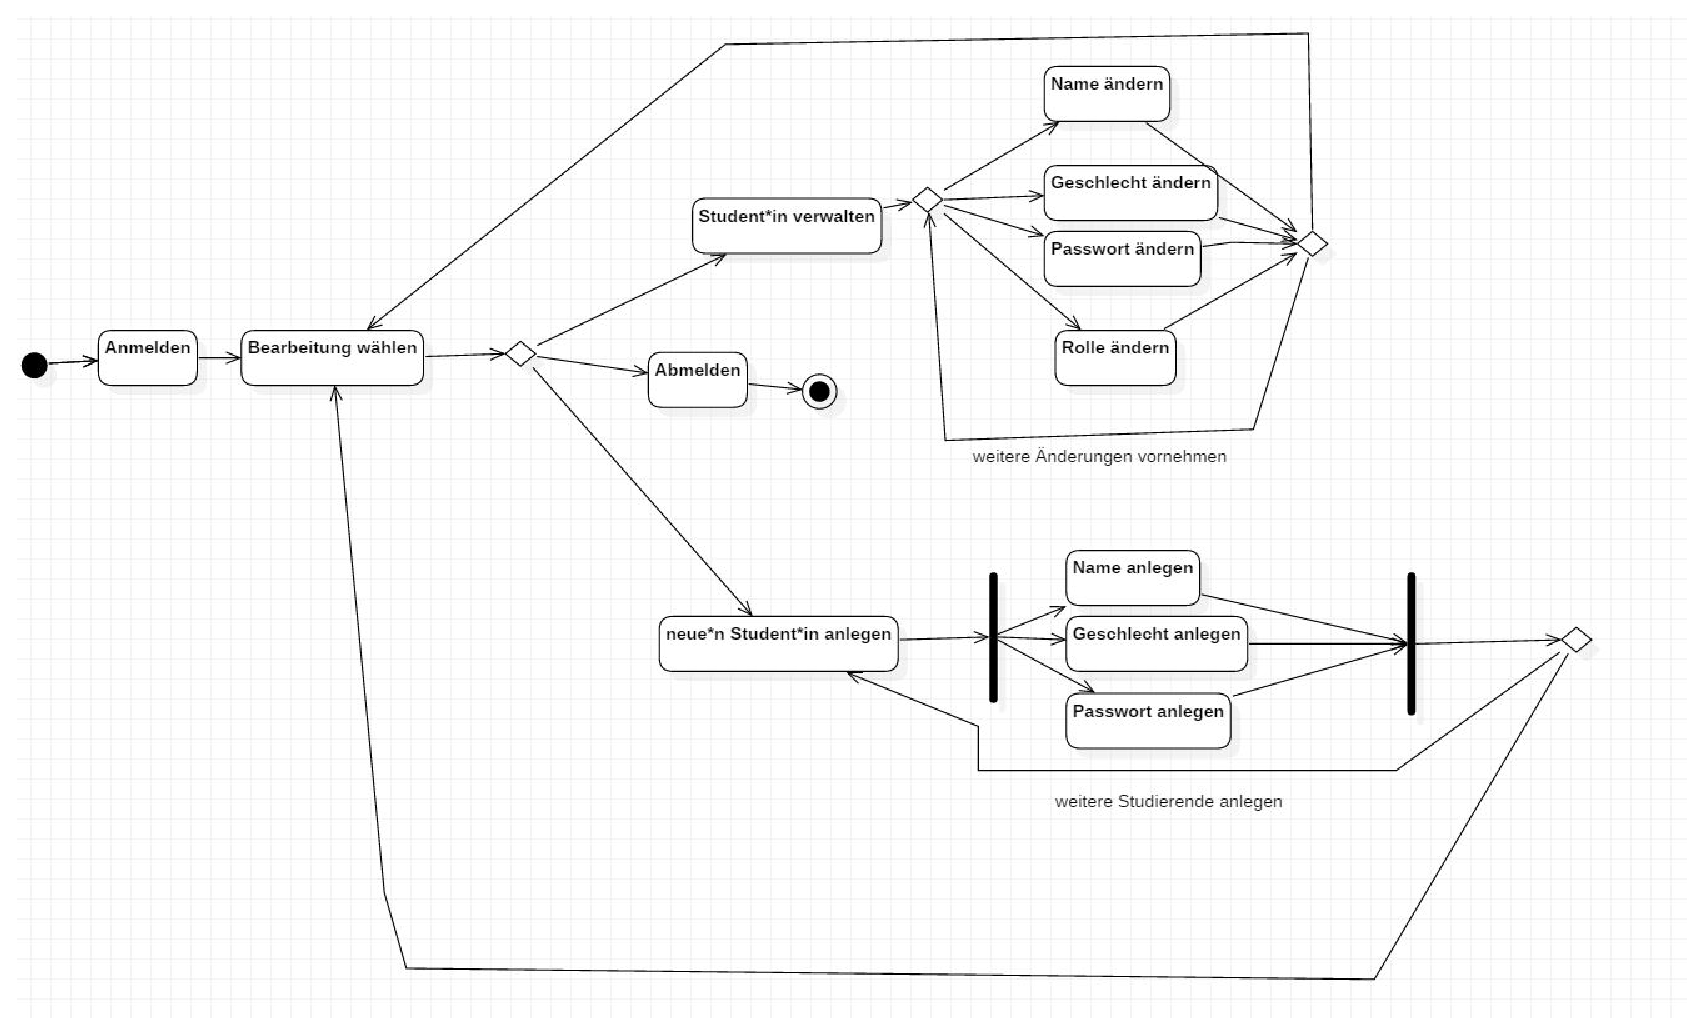
\includegraphics[width=1\linewidth]{pics/AdminE}
\caption[Admin]{UML Diagramm Administrationsoberfläche}
\label{fig:AdminE}
\end{figure}
\begin{figure}[!hbtp]%
\centering
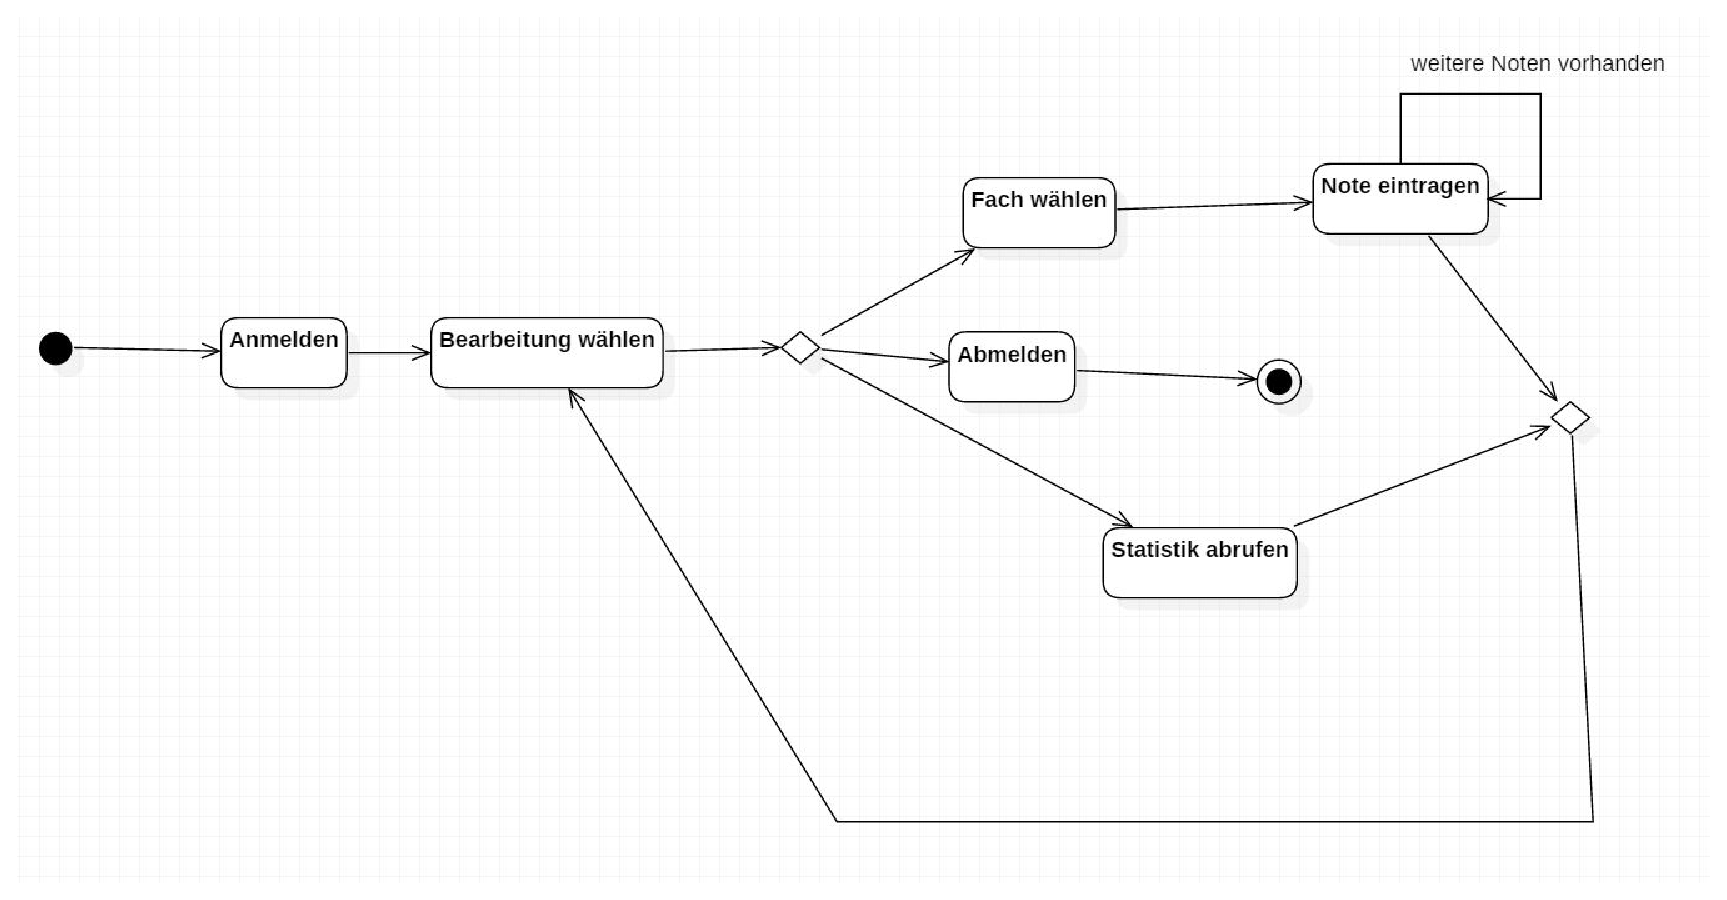
\includegraphics[width=1\linewidth]{pics/DozentIn}
\caption[Oberfläche Dozenten]{UML Diagramm Oberfläche Dozenten}
\label{fig:DozentIn}
\end{figure}
\begin{figure}
\centering
\includegraphics[width=1\linewidth]{pics/Schueler}
\caption[Oberfläche Student]{UML Diagramm Oberfläche Student}
\label{fig:Schueler}
\end{figure}
\section{Use Case Diagramme}
\begin{figure}[!h]
\centering
\includegraphics[width=1\linewidth]{pics/UseCase}
\caption[Use Case Diagramm]{Use Case Diagramm}
\label{fig:UseCase}
\end{figure}
\begin{figure}[!h]
\centering
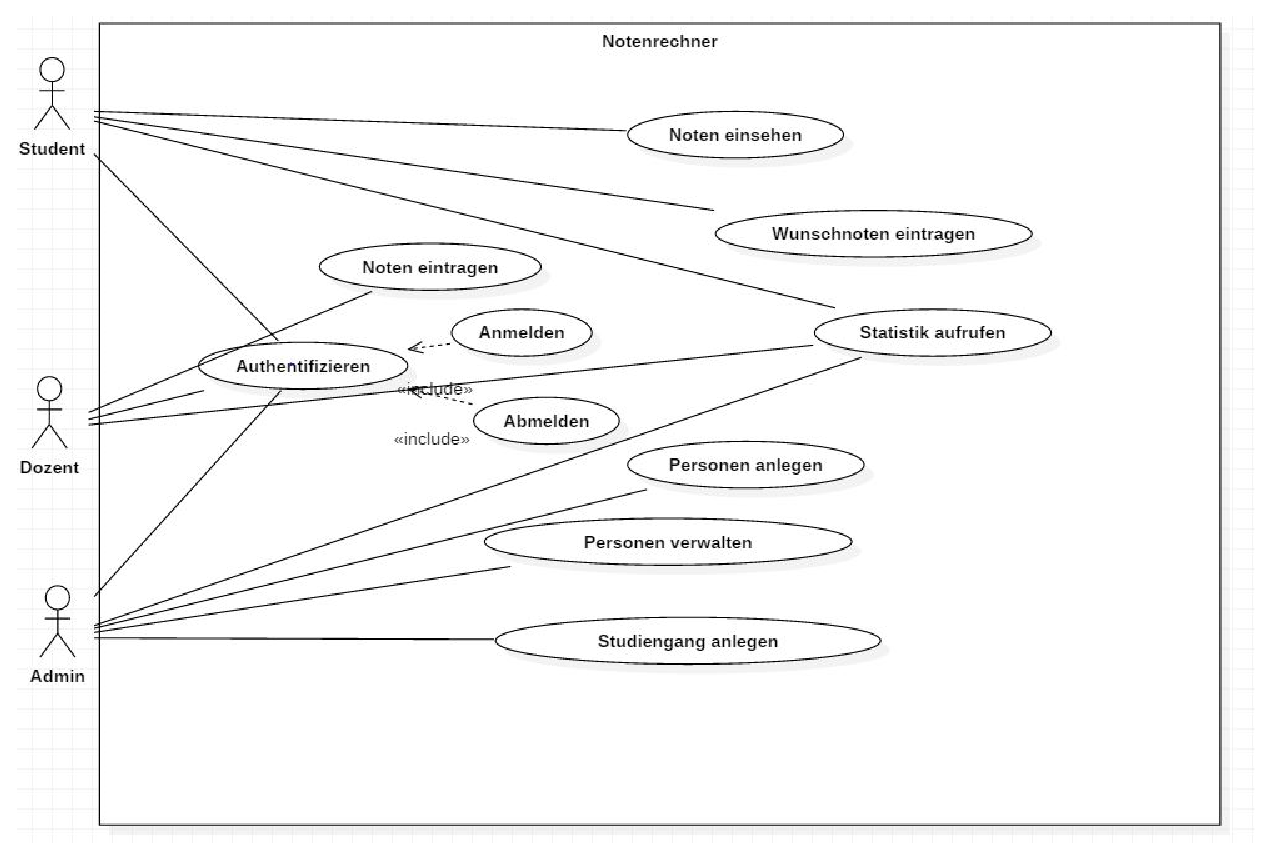
\includegraphics[width=1\linewidth]{pics/UseCase2}
\caption[Use Case Diagramm]{Use Case Diagramm 2}
\label{fig:UseCase2}
\end{figure}


\section{Klassendiagramme}
\begin{figure}[!h]
	\centering
	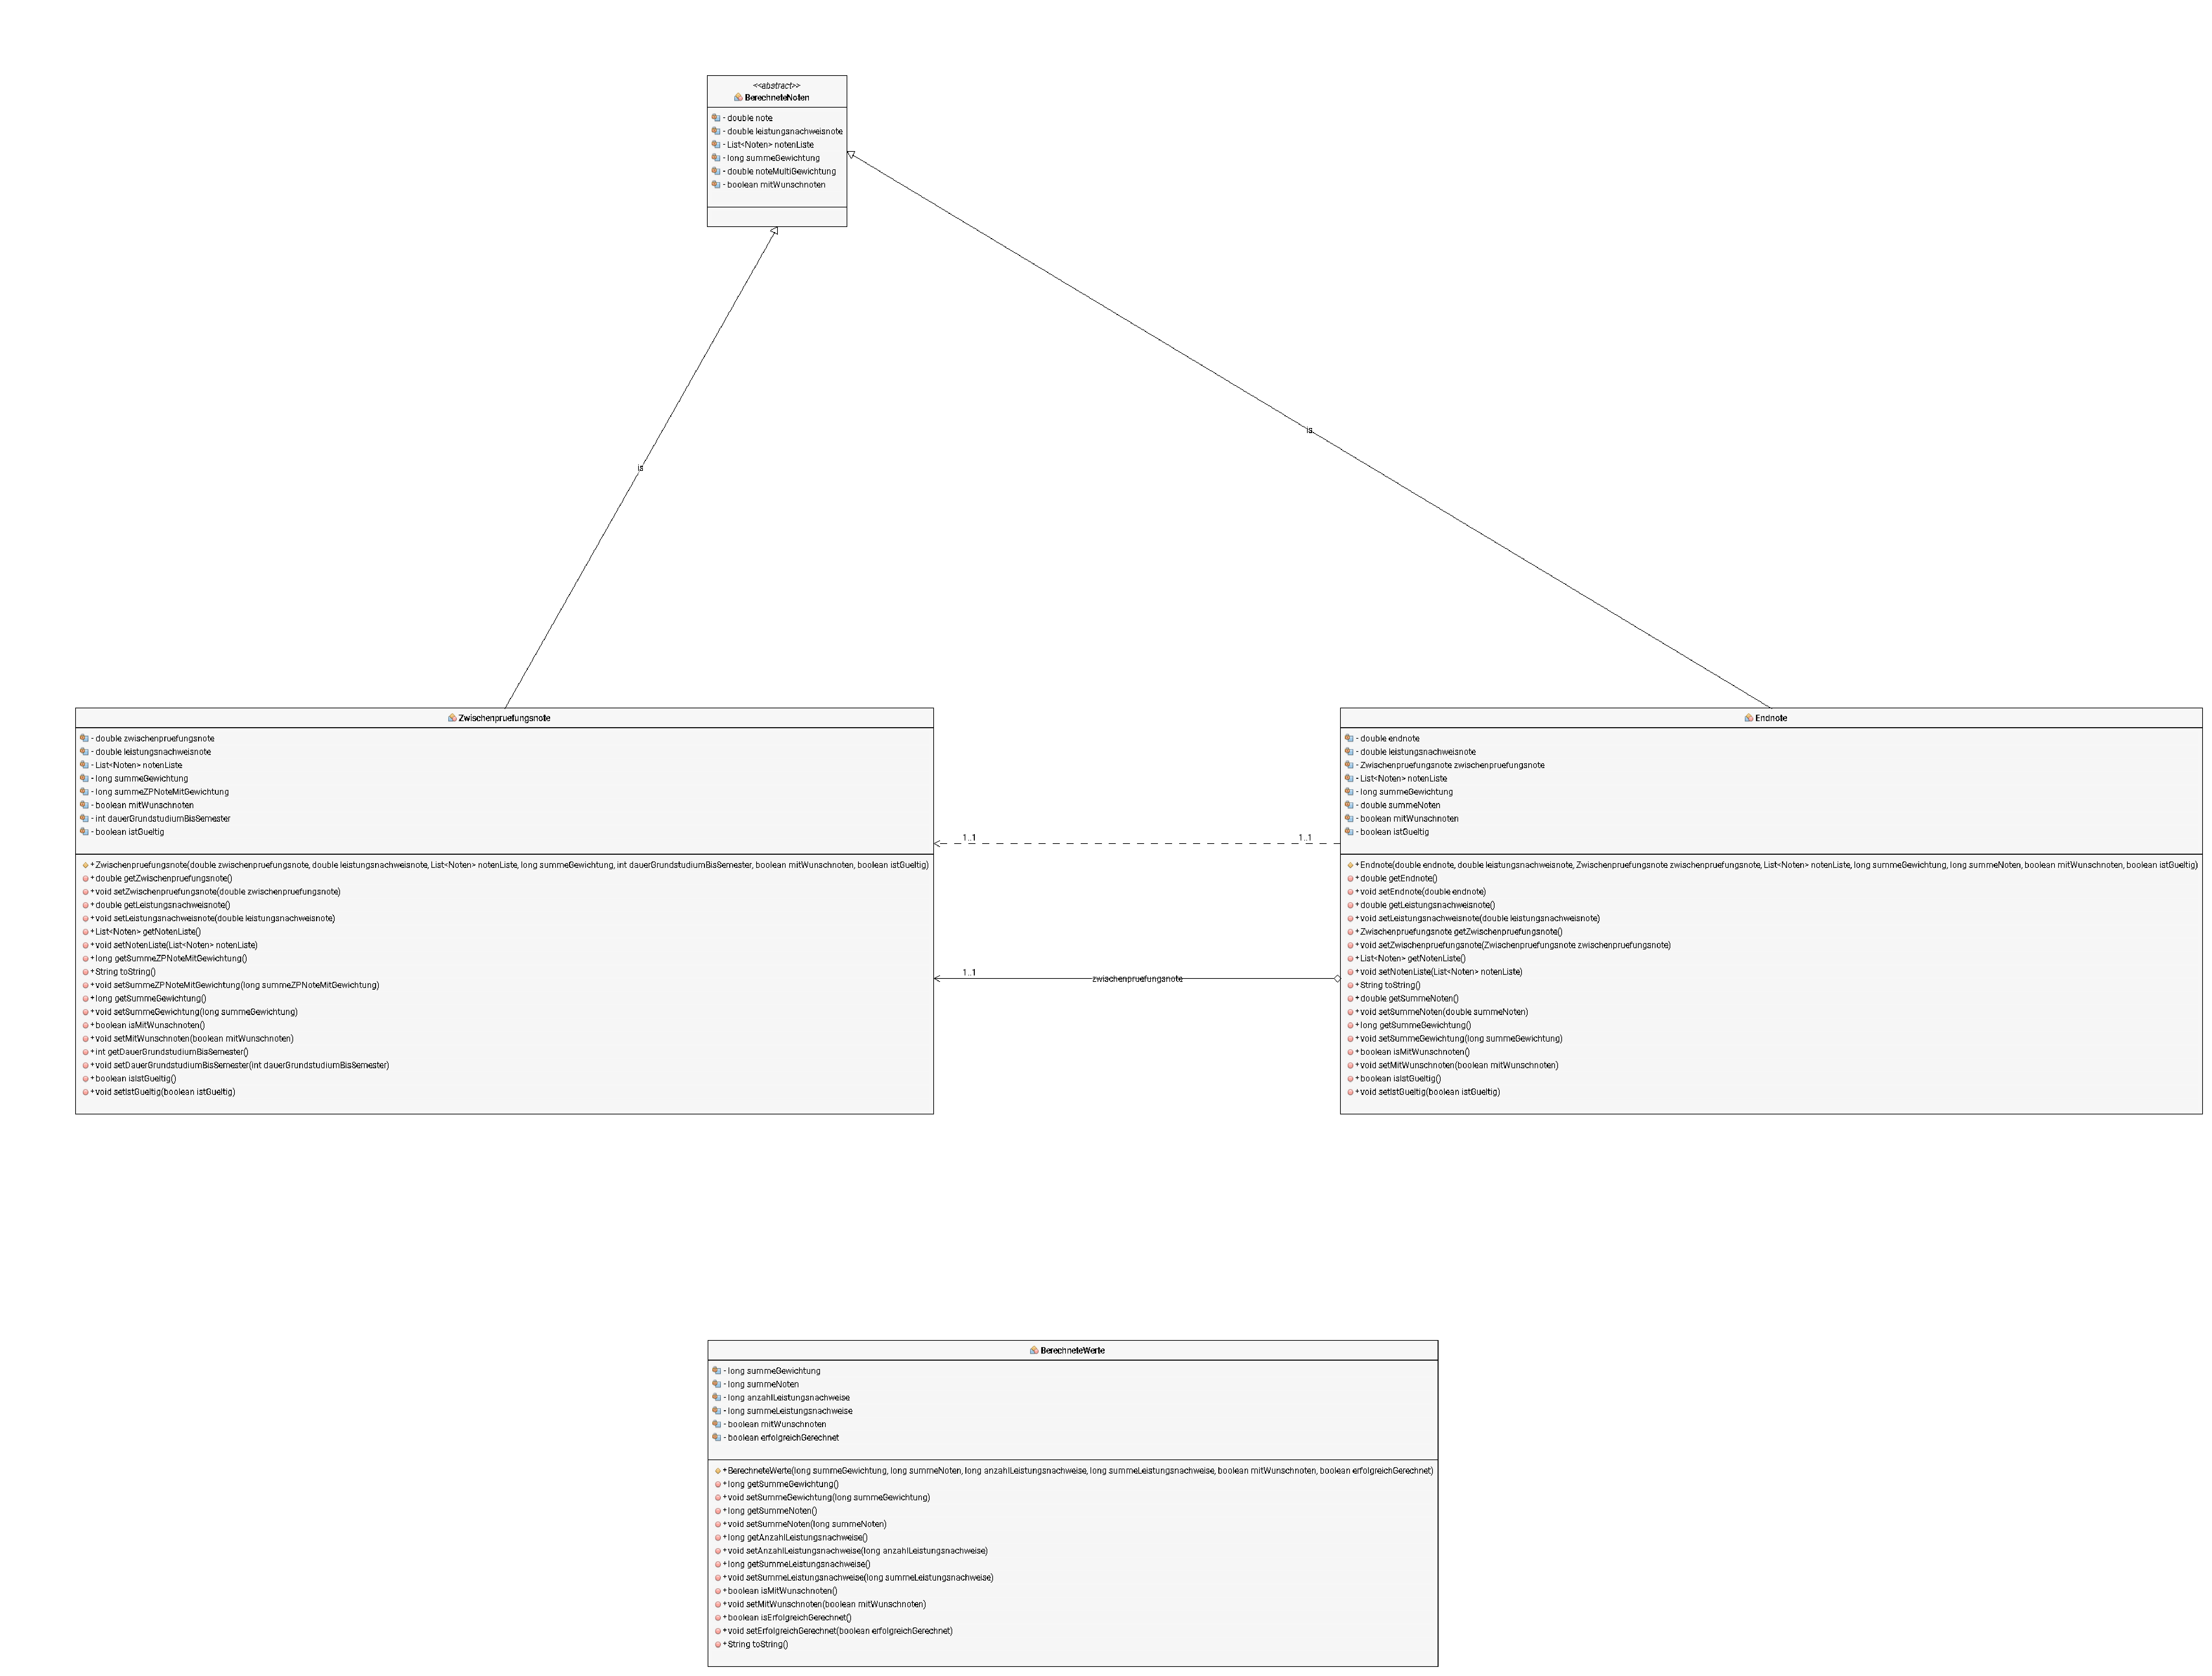
\includegraphics[width=1\linewidth]{Diagramme/generated/package_eigene_noten_autosortiert}
	\caption[Package Eigene Noten]{UML Klassendiagramm des Packages \glqq Eigene Noten\grqq}
	\label{fig:package_eigene_noten}
\end{figure}
\begin{figure}[!hbtp]%
	\centering
	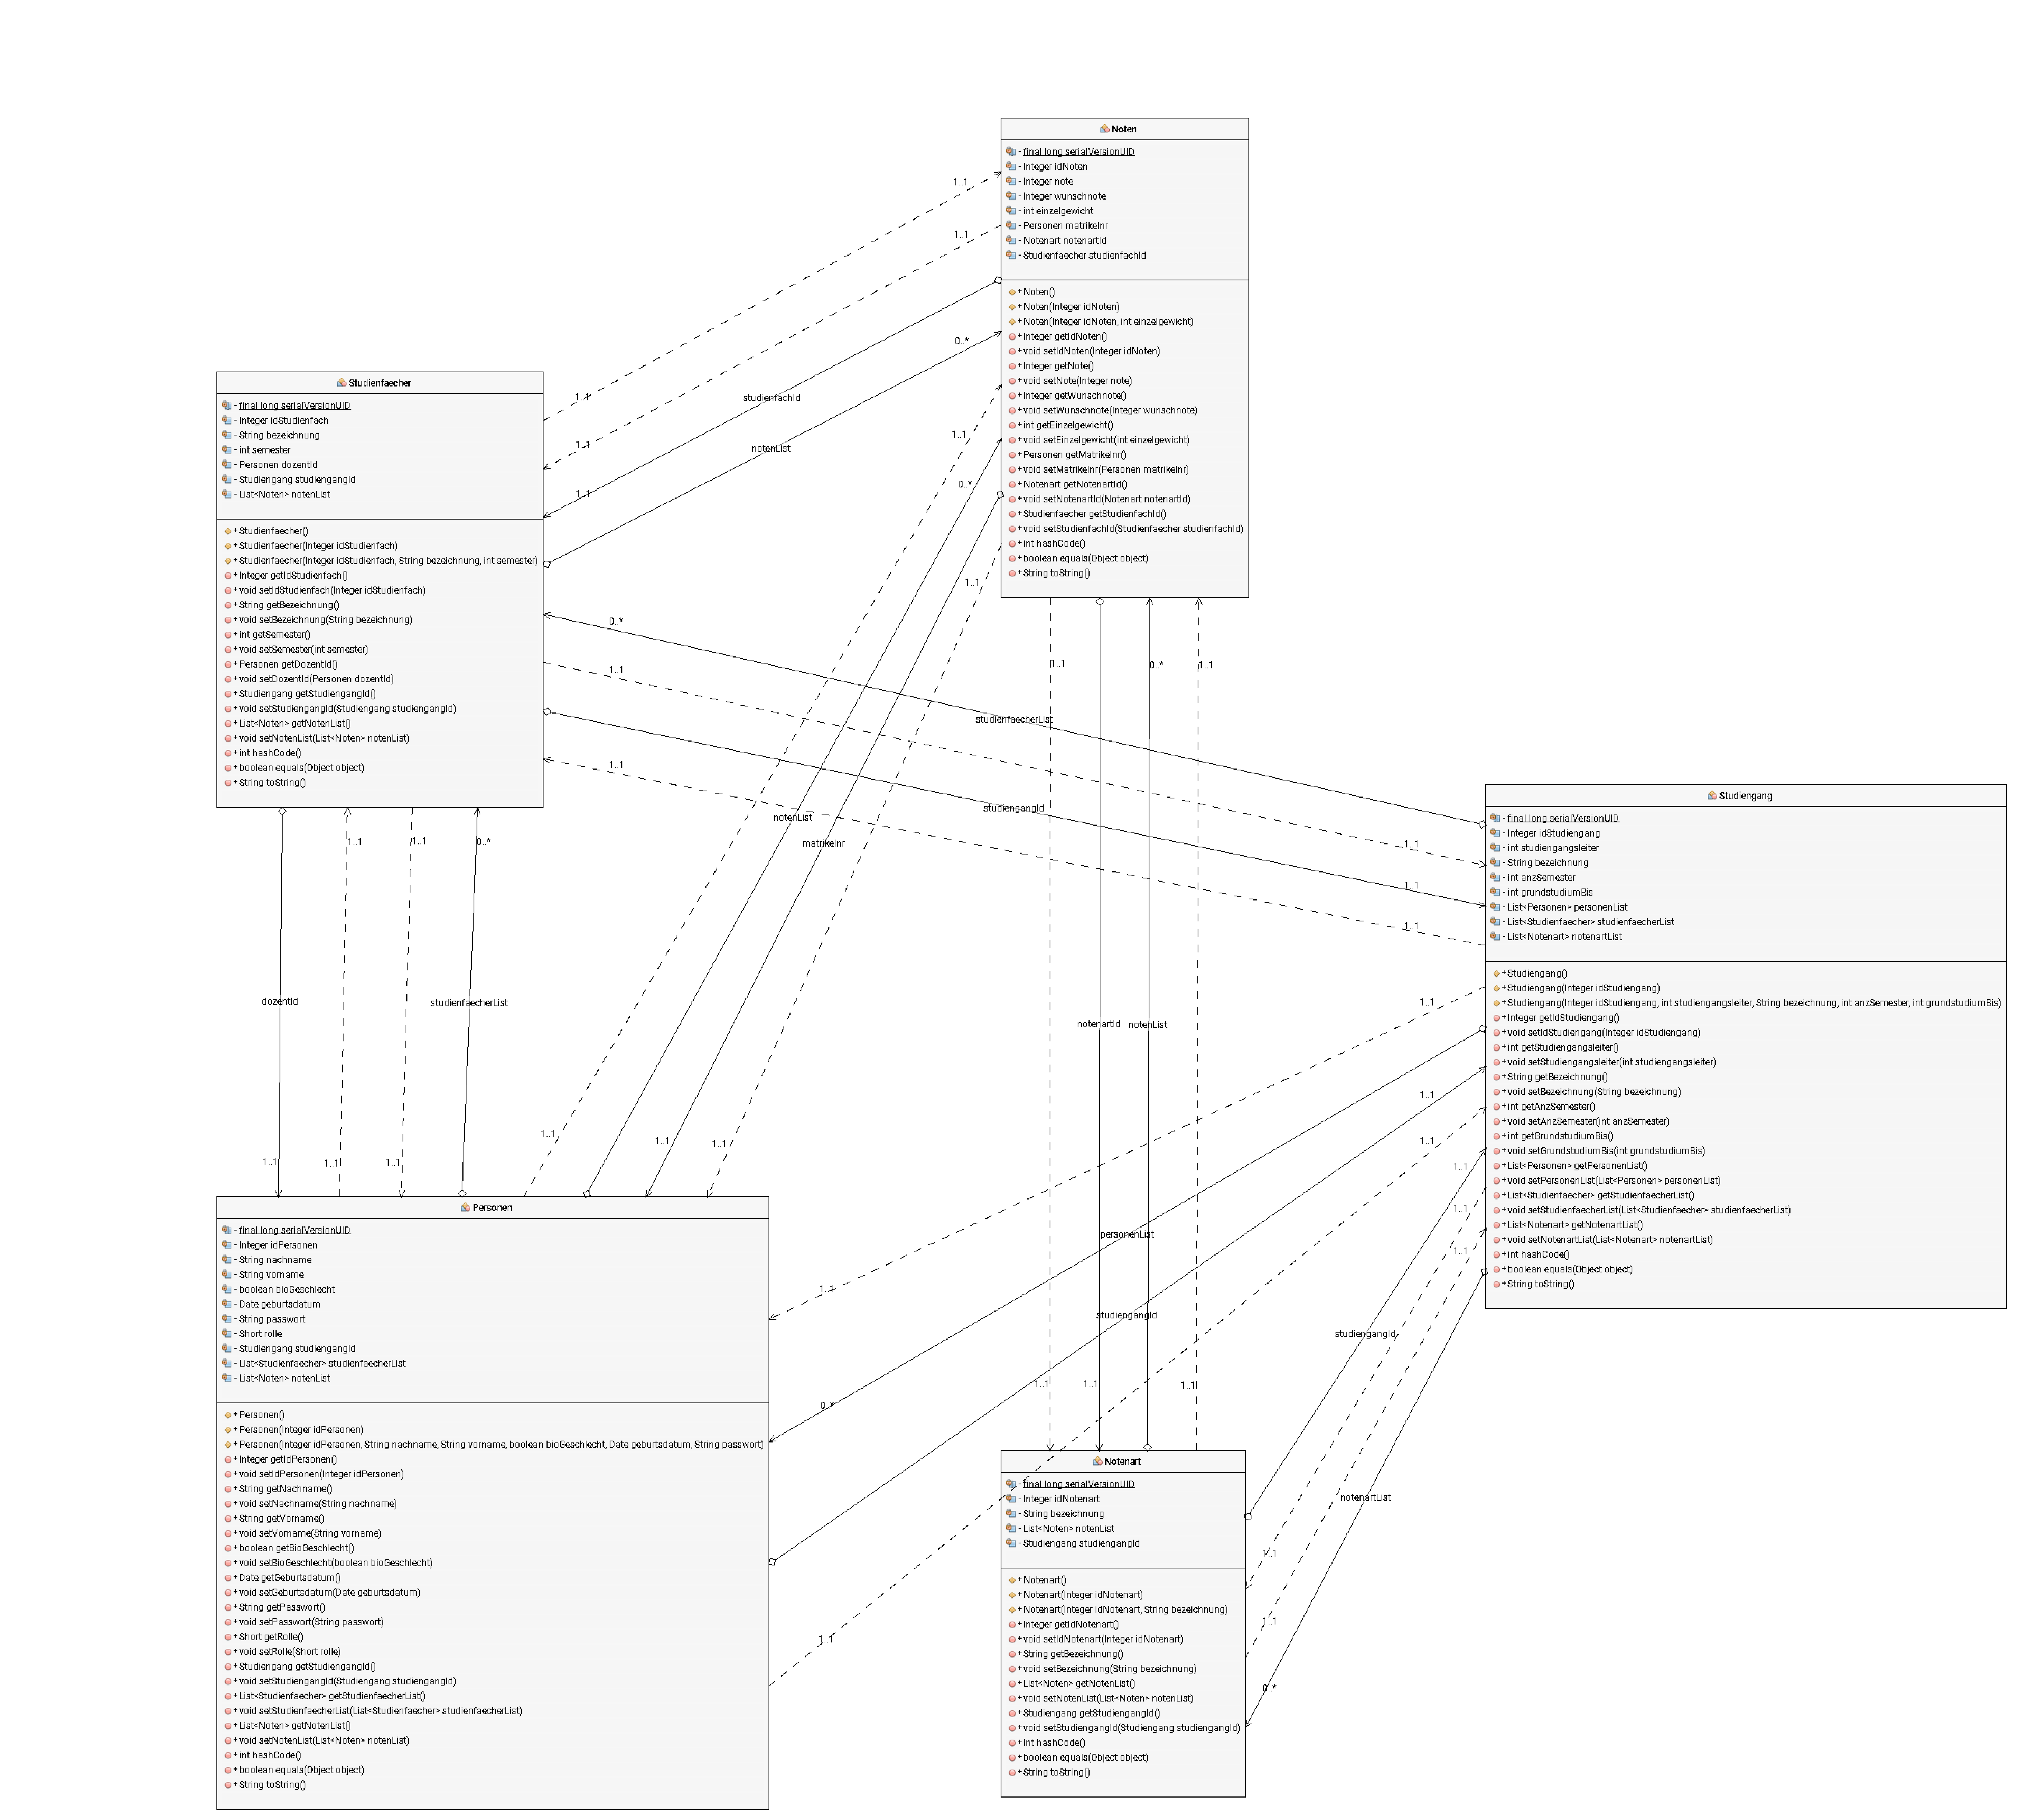
\includegraphics[width=1\linewidth]{Diagramme/generated/package_entity}
	\caption[Package Entity]{UML Klassendiagramm des Packages \glqq Entity\grqq}
	\label{fig:package_entity}
\end{figure}
\begin{figure}[!hbtp]%
	\centering
	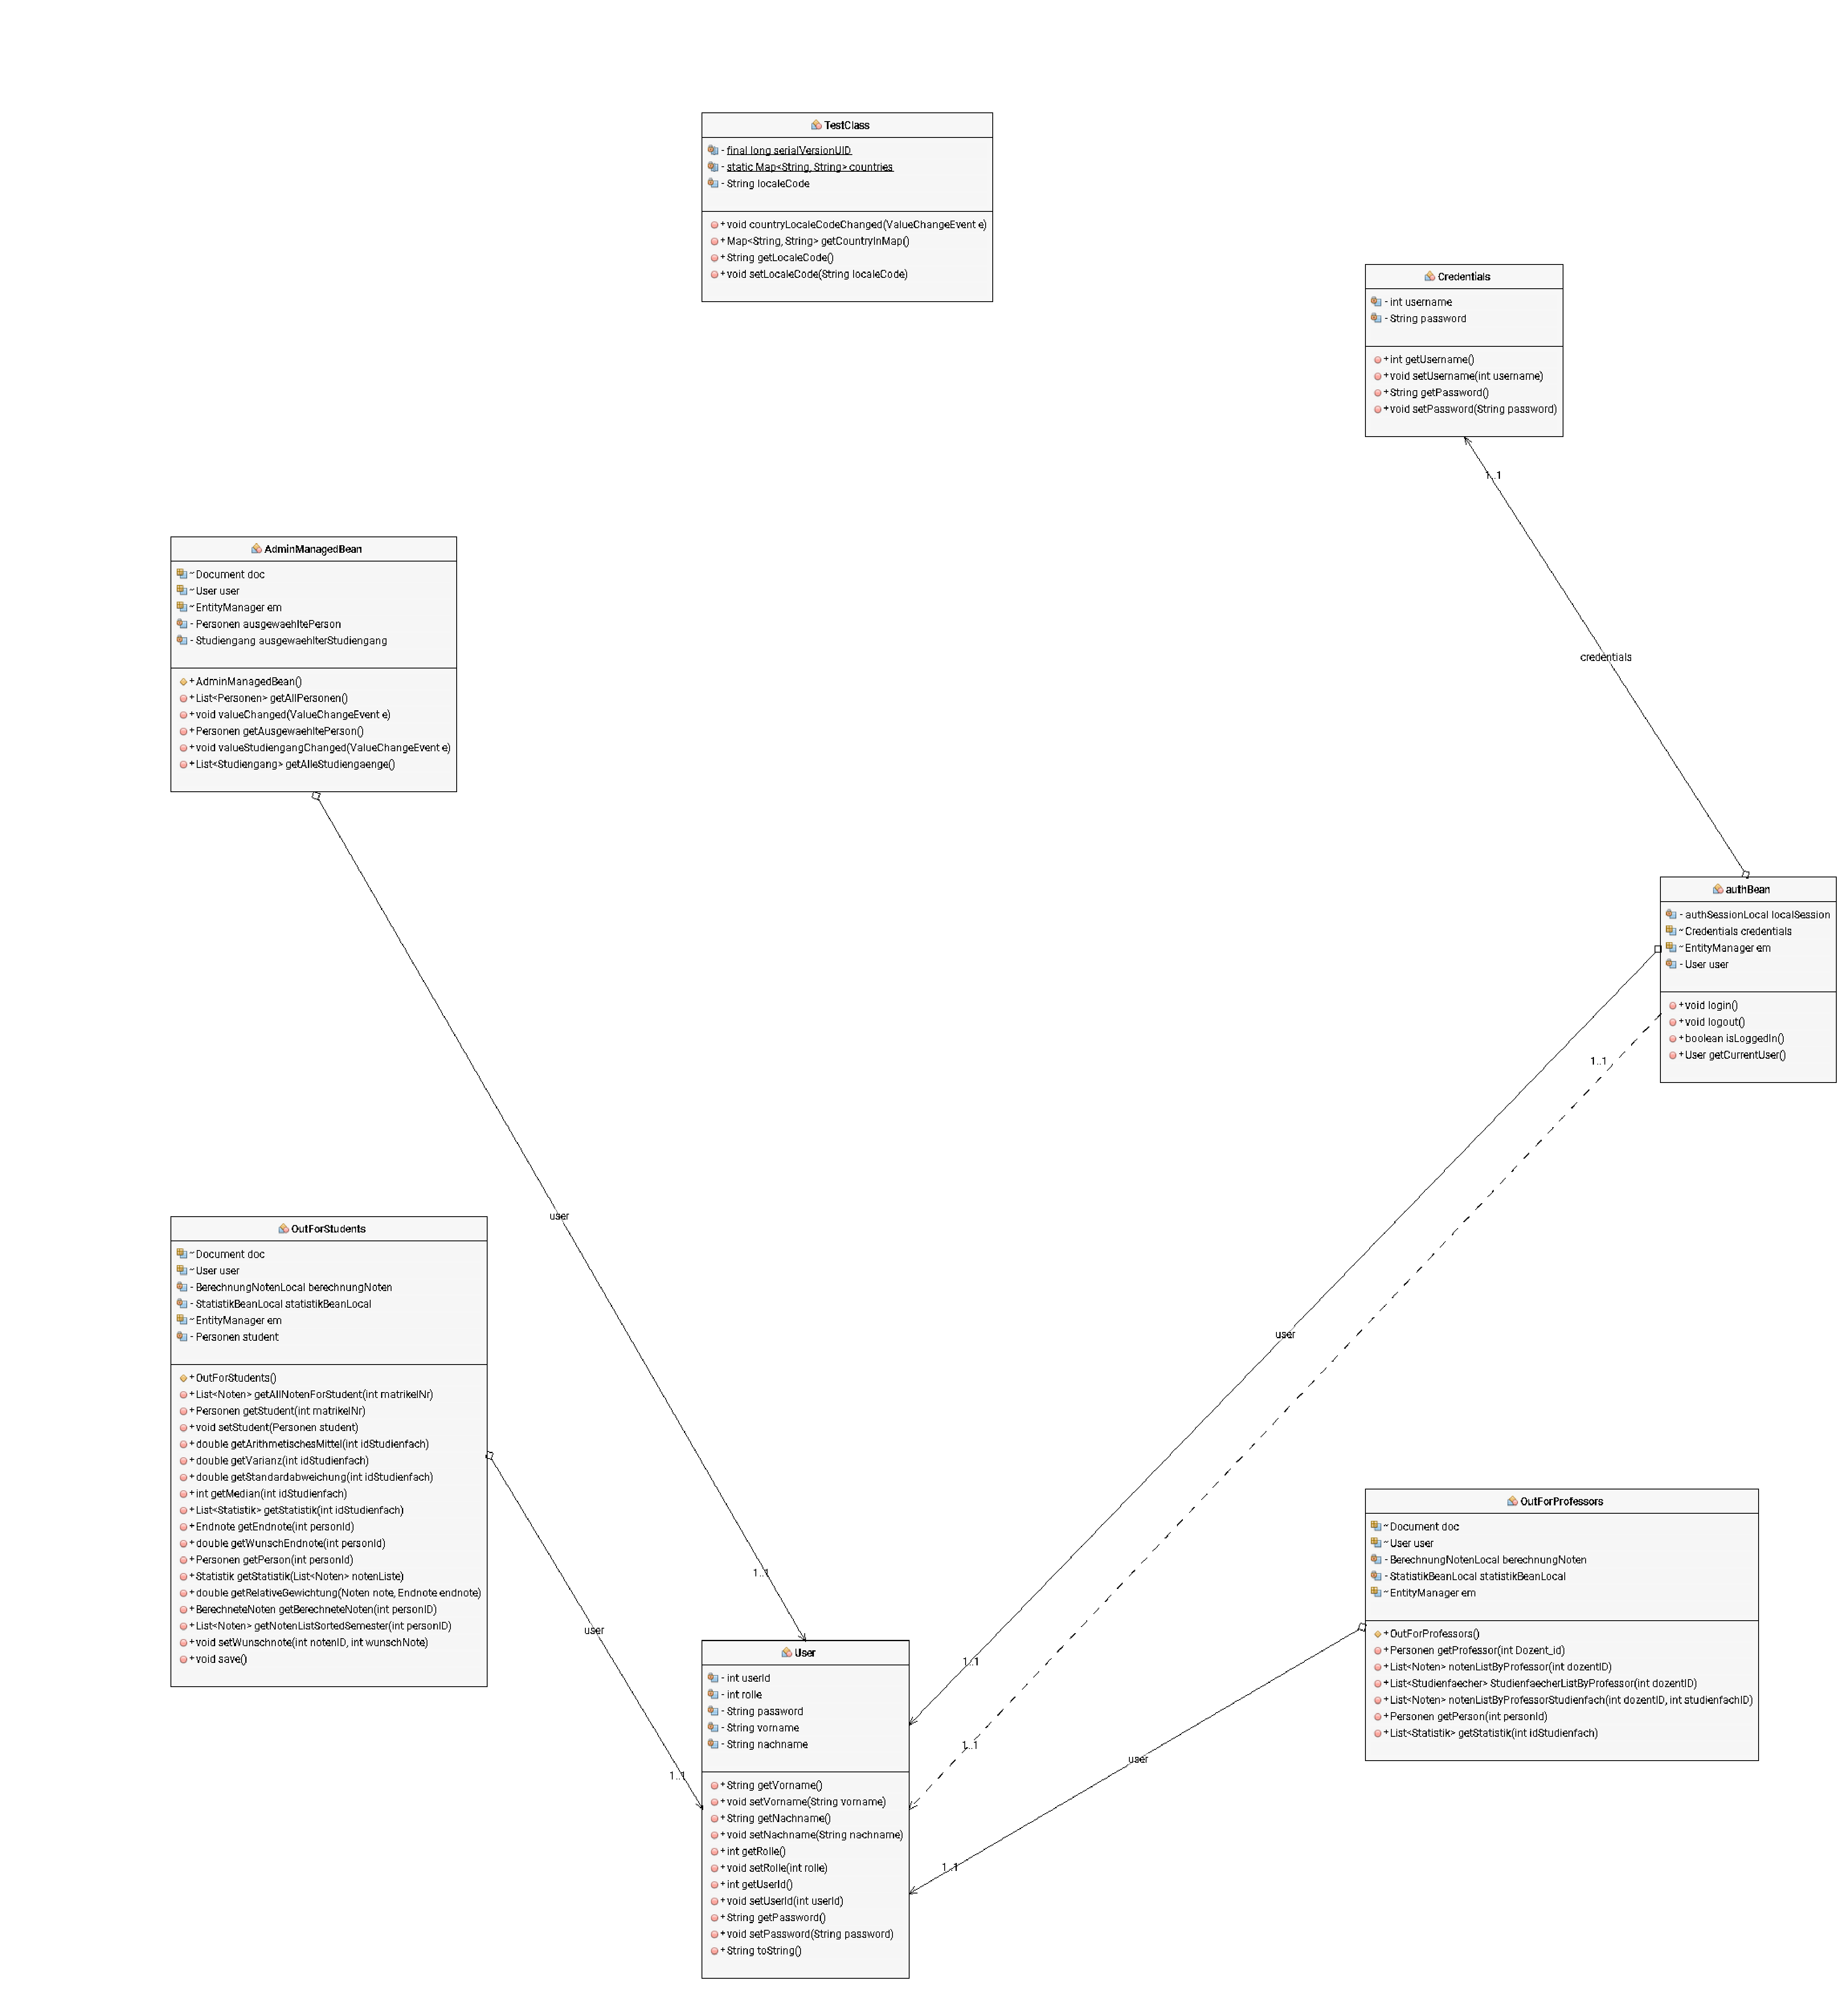
\includegraphics[width=1\linewidth]{Diagramme/generated/package_managedBean}
	\caption[Package Managed Bean]{UML Klassendiagramm des Packages \glqq Managed Bean\grqq}
	\label{fig:package_managed_bean}
\end{figure}
\begin{figure}[!hbtp]%
	\centering
	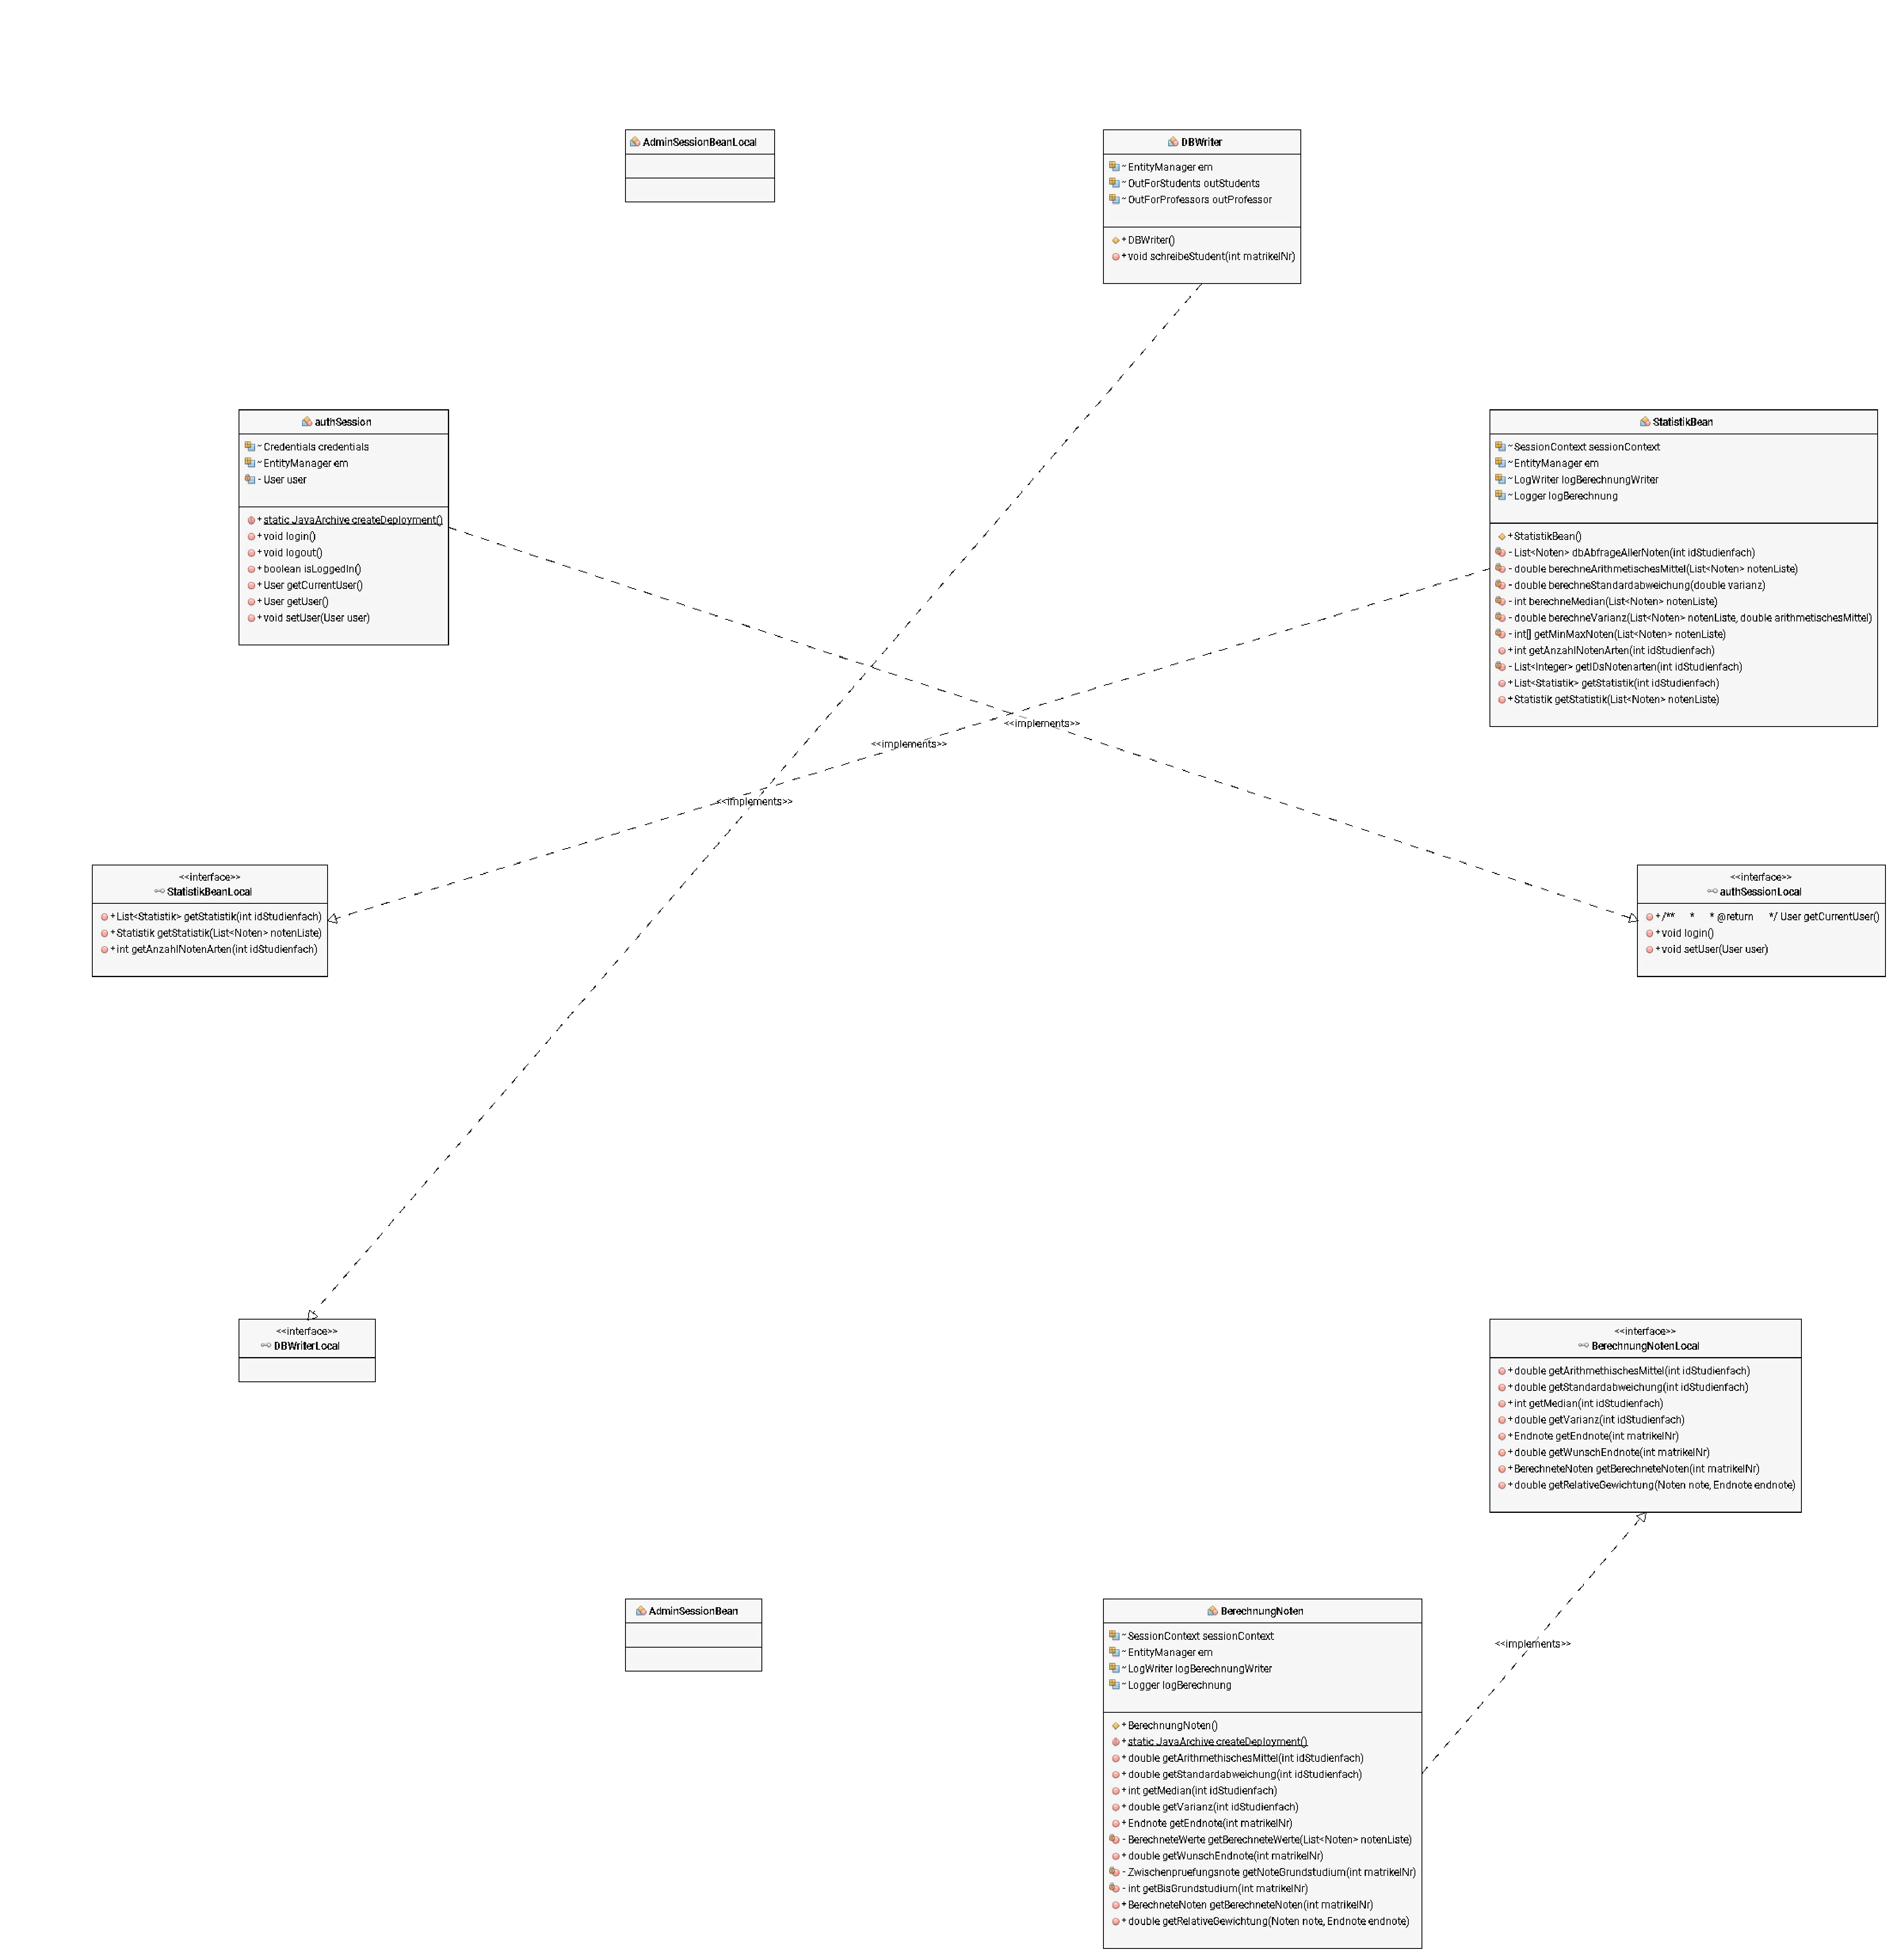
\includegraphics[width=1\linewidth]{Diagramme/generated/package_sessionBean}
	\caption[Package Session Bean]{UML Klassendiagramm des Packages \glqq Session Bean\grqq}
	\label{fig:package_session_bean}
\end{figure}
\begin{figure}[!hbtp]%
	\centering
	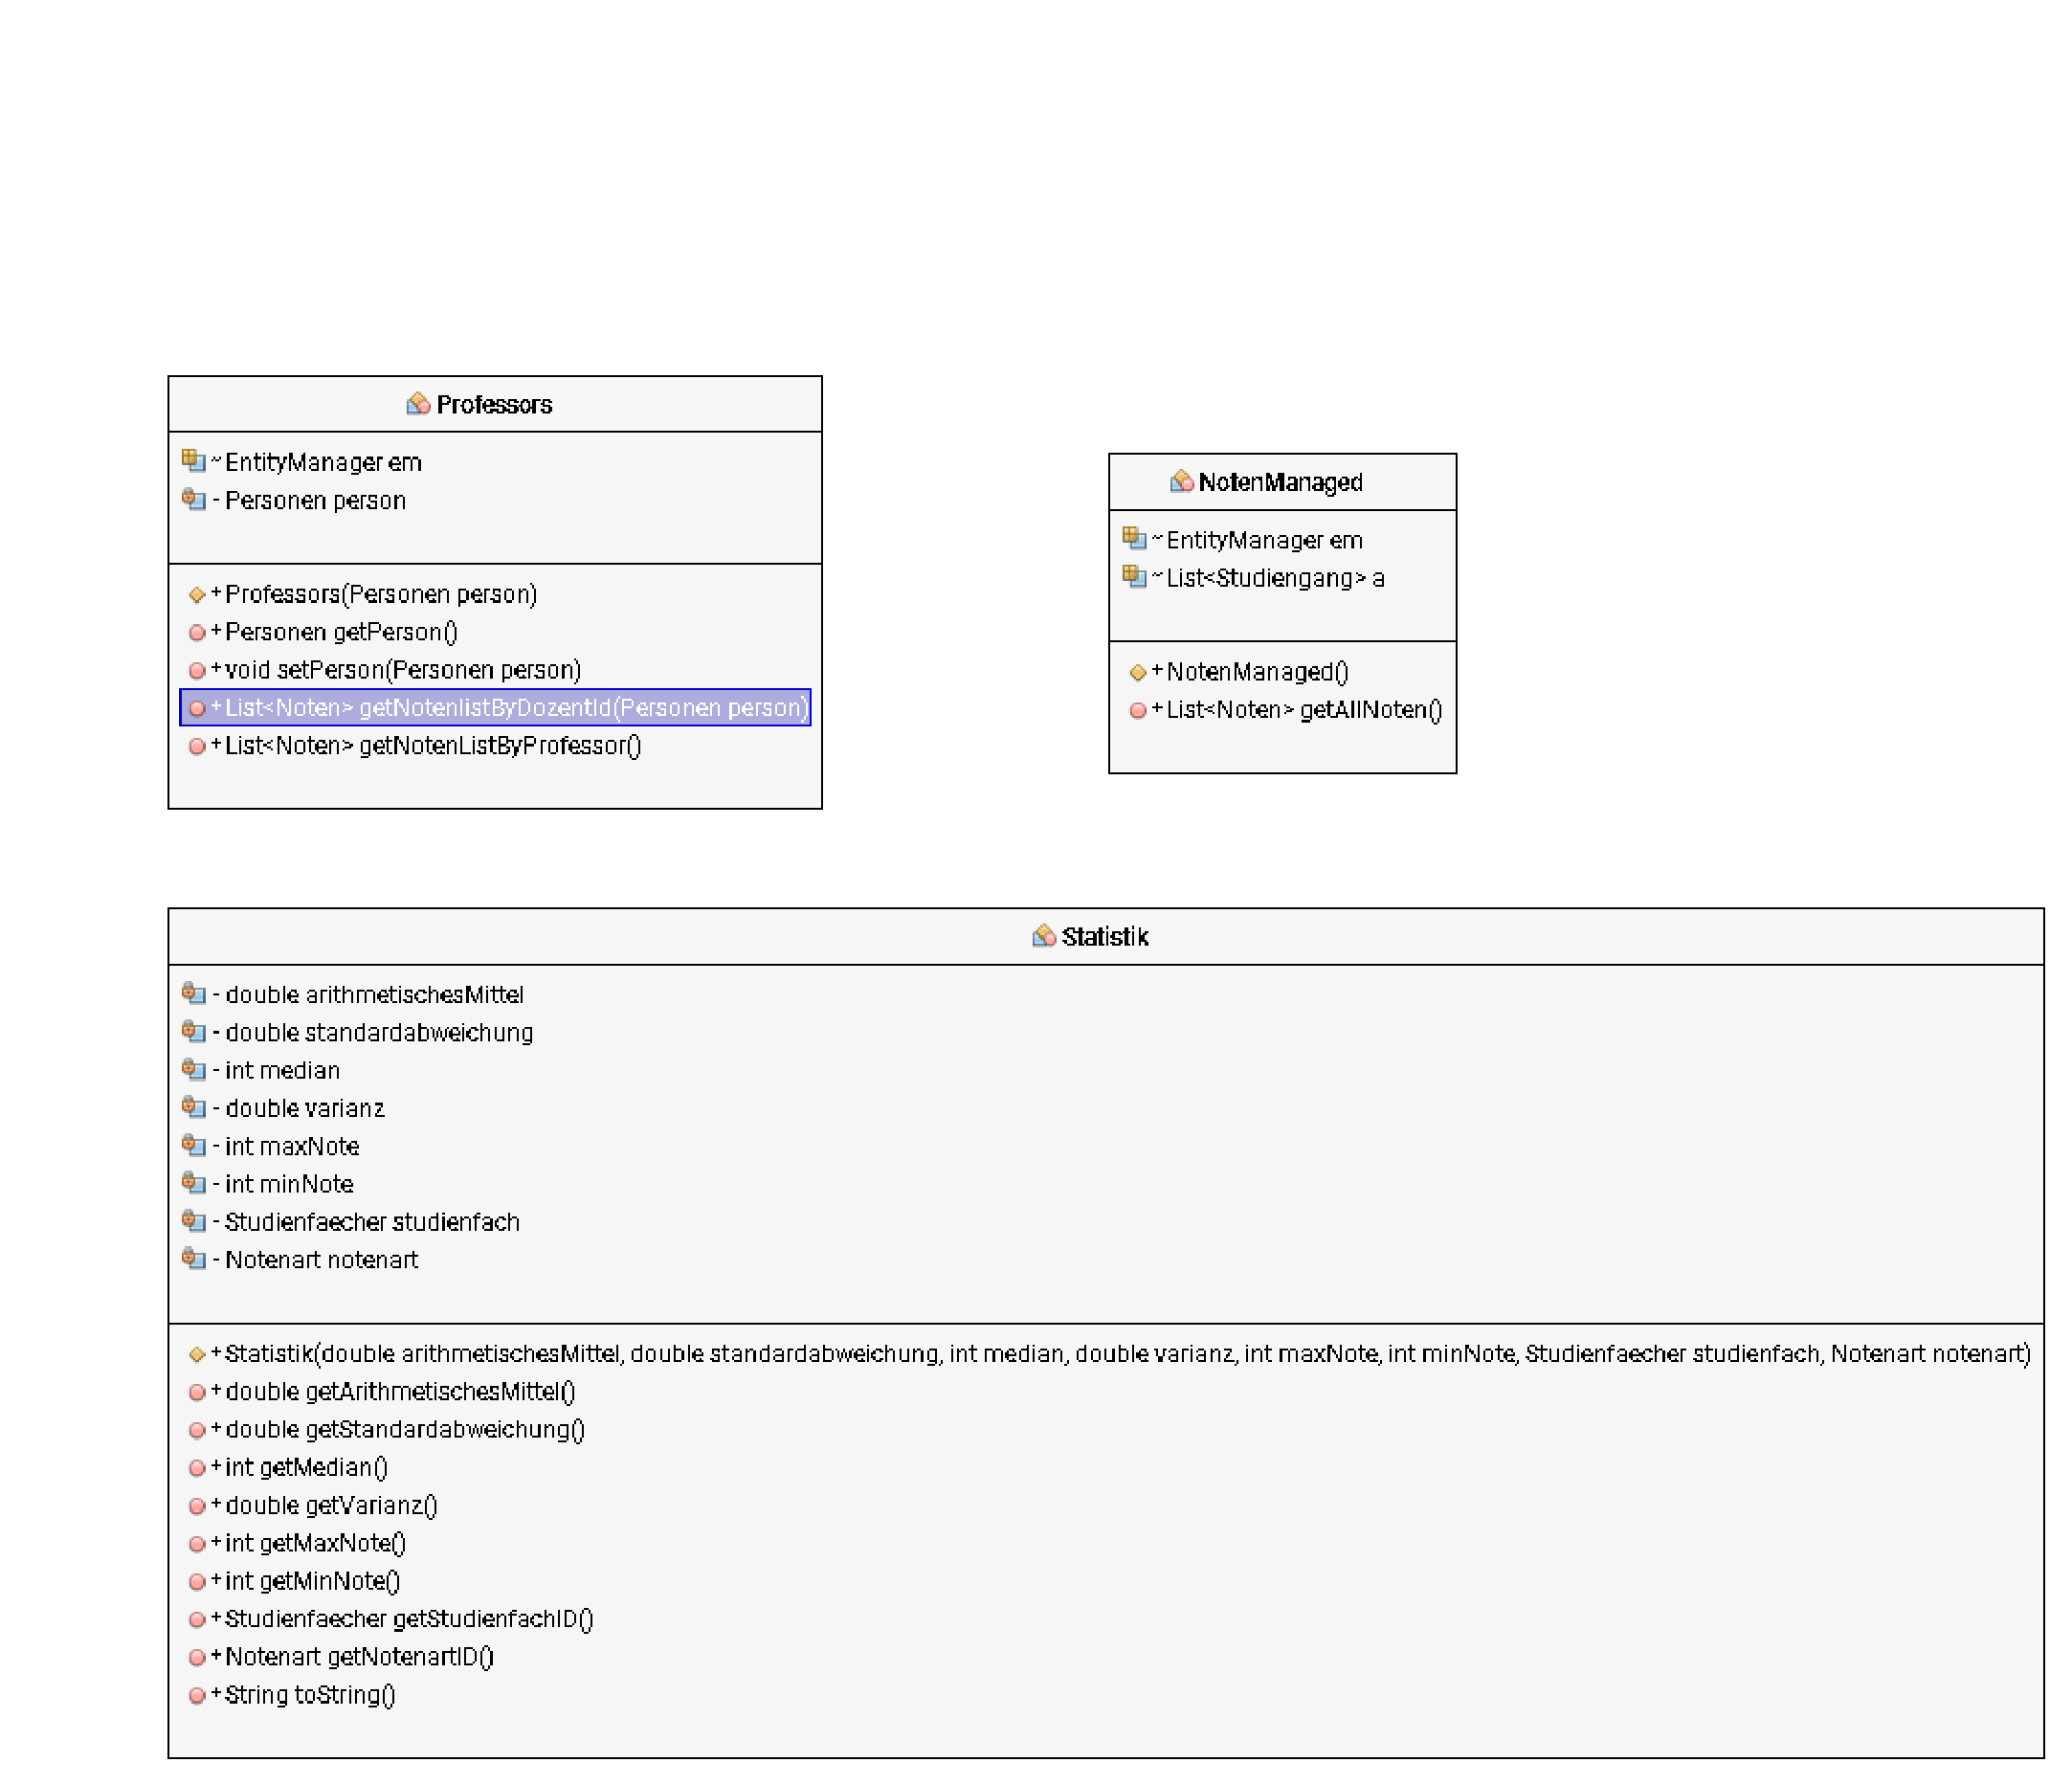
\includegraphics[width=1\linewidth]{Diagramme/generated/package_test}
	\caption[Package Test]{UML Klassendiagramm des Packages \glqq Test\grqq}
	\label{fig:package_test}
\end{figure}
\section{Datenbank Entity Relationship Diagramm}
\begin{figure}[!hbtp]%
\centering
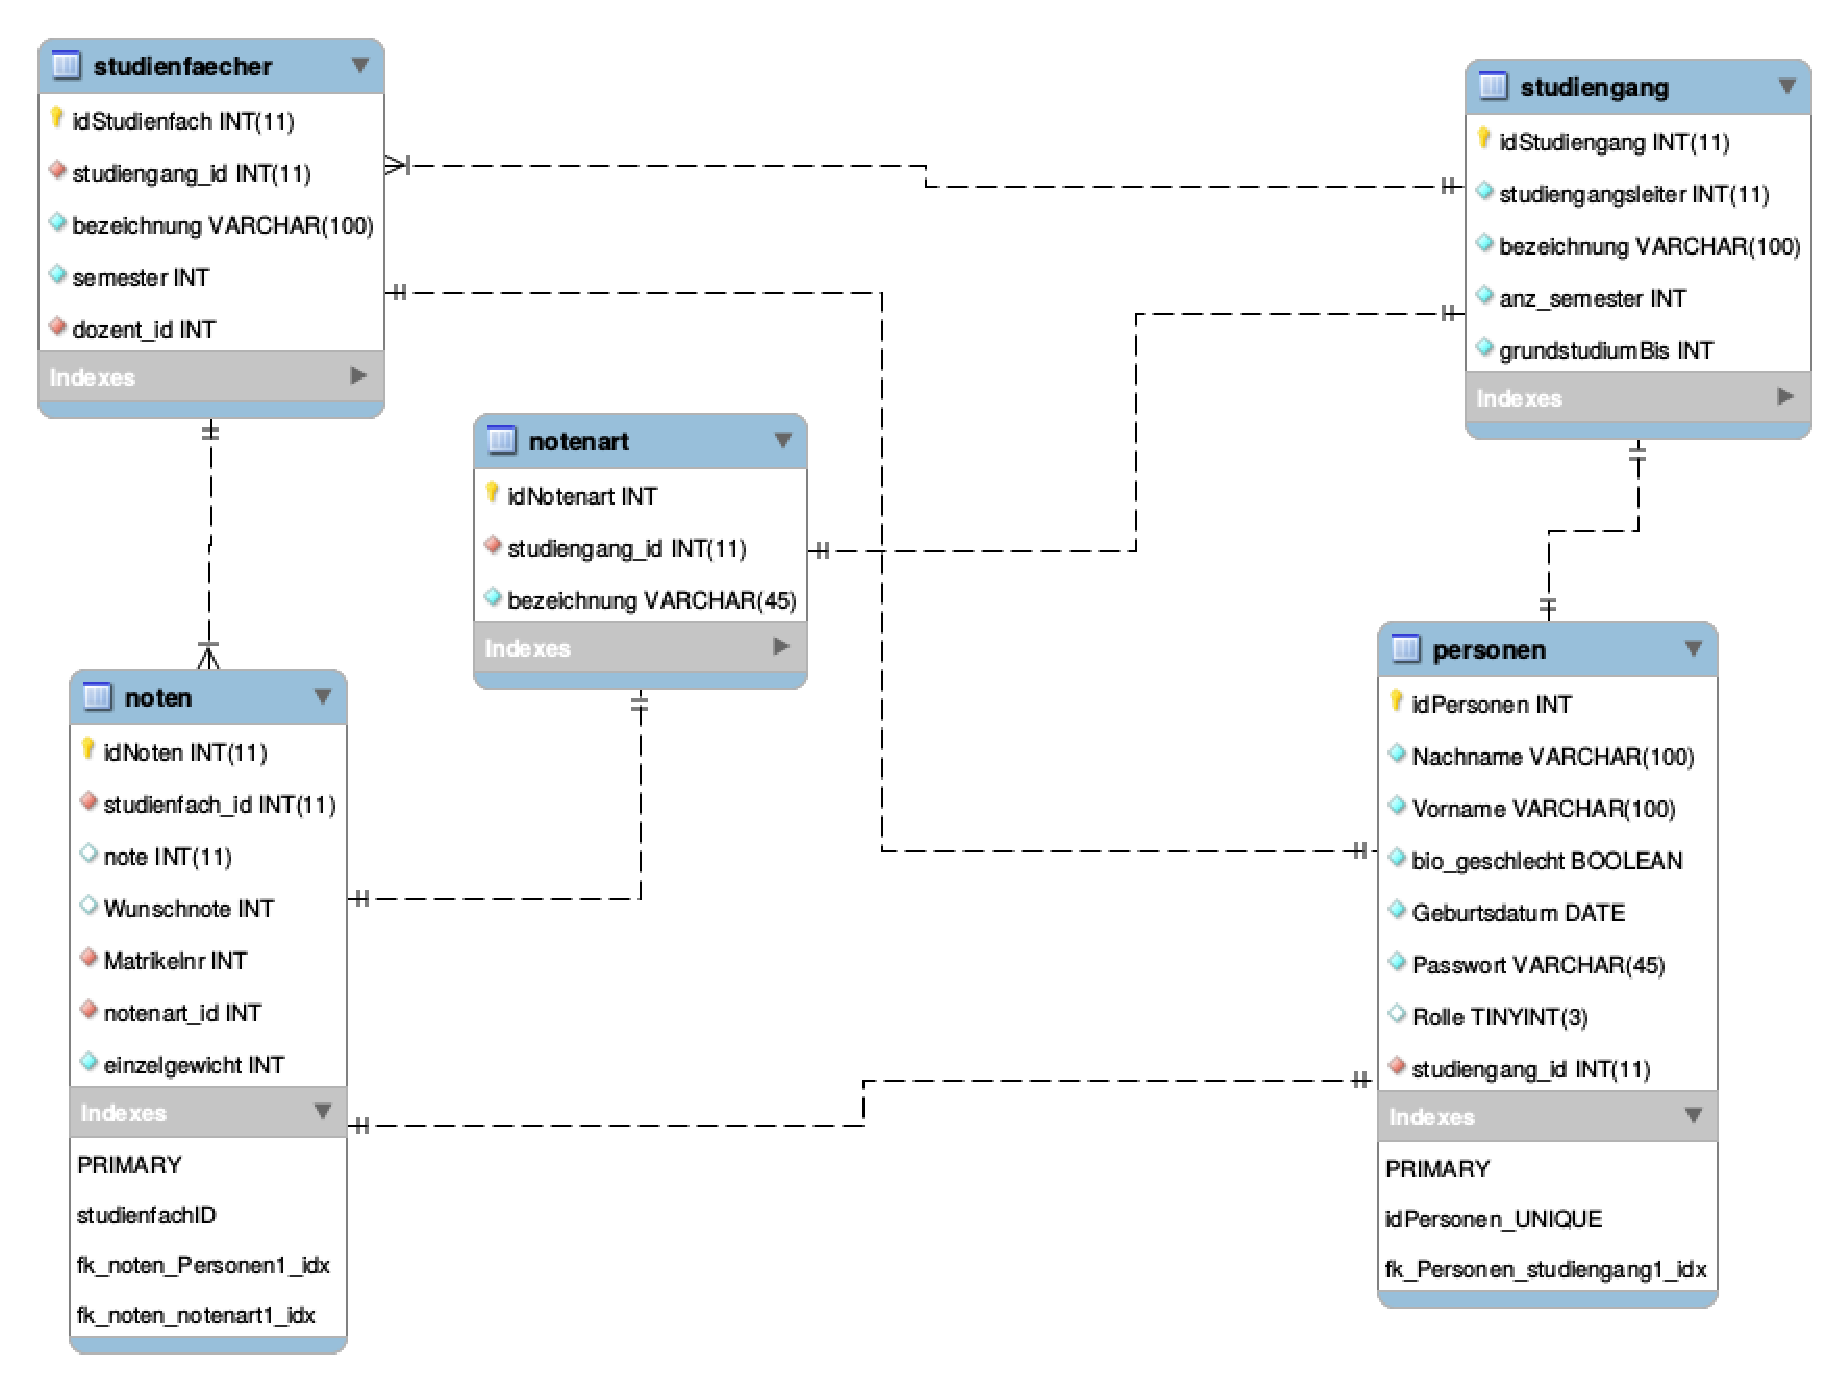
\includegraphics[width=1\linewidth]{pics/dbERModell}
\caption[ER Diagramm DB]{Entity Relationship Modell für die Datenbank}
\label{fig:dbERModell}
\end{figure}

%TODO Diagramme von Stefan
\listoffigures
\end{document}

